\newcommand{\tabBeitrag}{0.1\textwidth}
\newcommand{\tabOther}{0.2\textwidth}

\newcommand{\durchfuehrungsweg}{0.15\textwidth}
\newcommand{\finanzierung}{0.07\textwidth}
\newcommand{\tarife}{0.07\textwidth}
\newcommand{\beitrag}{0.3\textwidth}
\newcommand{\zuzahlung}{0.1\textwidth}
\newcommand{\bvierzig}{0.07\textwidth}
\newcommand{\bdreiEStG}{0.07\textwidth}


\newcommand{\bDrei}{0.24\textwidth}
\newcommand{\bZwei}{0.14\textwidth}
\newcommand{\bAlle}{0.54\textwidth}

\newcommand{\siebenTabBeitrag}{0.64\textwidth}
\newcommand{\tabTemp}{0.13\textwidth}

\newcommand{\values}{0.14\textwidth}

\newcommand{\tabComplex}{0.12\textwidth}

\newcommand{\tabRandom}{0.075\textwidth}

\newcolumntype{M}[1]{>{\centering\arraybackslash}m{#1}}

\chapter{Anwendungsfall}\label{chap:anwendungsfall}

Im folgenden Kapitel wird der Anwendungsfall vorgestellt, der als Grundlage zur Beantwortung der Fragestellungen dieser Arbeit (vgl. \autoref{sec:zielderArbeit}) dient. Der Anwendungsfall befasst sich mit der Untersuchung der Webanwendung Easy Web Leben \cite{easy_web}(\url{https://www.al-h.de/appserver/easyweb/}), im Folgenden Easy Web genannt. Die Plattform dient zur Erstellung von Angeboten im Bereich von Lebensversicherungsprodukten. Die Struktur dieses Kapitels sieht wie folgt aus: Zunächst werden einige relevante versicherungstechnische Begriffe eingeführt, anhand derer sich eine detaillierte Beschreibung der Easy Web-Plattform anschließt. Daraufhin wird die konkrete Methodik und Implementierung zur Beantwortung der Fragestellungen erläutert, zudem die Ergebnisse der korrespondierenden Untersuchungen vorgestellt.

\section{Vorstellung des Testobjekts}\label{sec:testobjekt}

Das 'Beratungscockpit' Easy Web \cite{easy_web} soll Vermittelnde und der Kundschaft der ALH-Gruppe bei der Ermittlung der individuellen Bedürfnisse im Bereich der Lebensversicherung unterstützen. Dafür steht eine Reihe verschiedener Produkte und Tarife zur Verfügung, die anhand unterschiedlicher Parameter an die individuellen Anforderungen der Kundschaft angepasst werden können und letztlich in einem konkreten Antrag zum Abschluss einer Versicherung münden können. Easy Web ermittelt parallel dazu anhand der eingegebenen Parameter verschiedene Komponenten des resultierenden Versicherungstarifs wie den Beitragsverlauf, Kapitalzahlungen, Todesfallleistungen, zugehörige Rentenleistung, etc.

Easy Web unterscheidet grundlegend zwischen Produkten der privaten Vorsorge und der betrieblichen Altersvorsorge (bAV). Der Anwendungsfall dieser Arbeit fokussiert sich auf den Bereich der bAV.

\subsection{Versicherungstechnische Grundlagen}\label{subsec:versicherungsgrundlagen}

Die betriebliche Altersvorsorge (bAV) hat im deutschen Rentensystem gemeinsam mit der gesetzlichen und der privaten Vorsorge das Ziel, zu 'einer angemessenen Gesamtversorgung beim Ausscheiden aus dem Arbeitsleben' \cite[S. 12]{buttler2017einfuehrung} jeder Person beizutragen. Die gesetzliche, private und betriebliche Altersvorsorge werden in diesem Zusammenhang auch häufig als die drei Säulen des deutschen Rentensystems bezeichnet \cite[S. 3]{plato2016betriebliche}. 

Der Begriff der bAV beinhaltet 'alle Leistungen, die einem Arbeitnehmer zur Altersvorsorge, Hinterbliebenenversorgung oder Invaliditätsversorgung von seinem Arbeitgeber aus Anlass des Arbeitsverhältnisses zugesagt worden sind' \cite[S. 1]{buttler2017einfuehrung}. Klassischerweise ermöglicht die bAV lebenslängliches Einkommen in der Rente, sichert also ein Langlebigkeitsrisiko ab. Es können aber auch biometrische Risiken abgesichert werden, wie beispielsweise bei Berufsunfähigkeits-, Erwerbsunfähigkeits- und Risikolebensversicherungen. 

Ursprünglich wurde die bAV als 'zusätzliche Sozialleistung des Arbeitgebers' \cite[S. 7]{buttler2017einfuehrung} eingeführt, sodass die Finanzierung der bAV aus wirtschaftlicher Sicht einzig über separate Beiträge des Arbeitgebers erfolgte (Arbeitgeber-finanziert). Seit dem Jahr 2002 besitzt jeder Arbeitnehmer das Recht auf Umwandlung seines Lohnes für die Nutzung einer bAV \cite[S. 23]{buttler2017einfuehrung}, zudem muss dieses Vorhaben vom Arbeitgeber nach § 1 a BetrAVG mit einem Zuschuss unterstützt werden \cite[S. 29]{buttler2017einfuehrung}, falls dieser Sozialversicherungsbeiträge durch die Entgeldumwandlung einspart. Steuert der Arbeitgeber nur den gesetzlich verpflichtenden Teil zur Entgeldumwandlung des Arbeitnehmers bei, spricht man von einer Arbeitnehmer-finanzierten bAV. Leistet der Arbeitgeber im Rahmen einer Entgeldumwandlung des Arbeitnehmers Beiträge zur bAV über den verpflichtenden Teil hinaus, so erfolgt die Finanzierung der bAV als sogenannte Misch-Finanzierung.

Für die konkrete Ausgestaltung einer bAV stehen verschiedene Durchführungswege zur Verfügung, die im Folgenden basierend auf Buttler und Keller \cite{buttler2017einfuehrung} vorgestellt werden:

\paragraph*{Direktzusage}
Bei der Direktzusage übernimmt der Arbeitgeber die unmittelbare Verantwortung für die mit dem Arbeitnehmer getroffenen Vereinbarungen über die Erbringung einer Vorsorgeleistung. Der Arbeitnehmer besitzt einen Rechtsanspruch auf die versprochene Leistung gegenüber dem Arbeitgeber. Diesen weist der Arbeitgeber in seiner Bilanz als Pensionsrückstellungen aus. Zusätzlich kann der Arbeitgeber die versprochenen Leistungen über eine Rückdeckungsversicherung absichern. Finanziert wird die Direktzusage üblicherweise durch den Arbeitgeber  (Arbeitgeber-finanziert), eine Entgeldwandlung ist jedoch auch möglich (Arbeitnehmer-finanziert) \cite[S. 140]{buttler2017einfuehrung}.

\paragraph*{Direktversicherung}

Die Direktversicherung beschreibt das Vorgehen, bei welchem der Arbeitgeber eine Lebensversicherung auf das Leben des Arbeitnehmers bei einer Lebensversicherungsgesellschaft abschließt und die Beiträge übermittelt. Versicherungsnehmer ist somit der Arbeitgeber, bezugsberechtigt für die abgeschlossene Versicherungsleistung sind jedoch der Arbeitnehmer beziehungsweise dessen Hinterbliebene. Finanziert wird die Direktversicherung allein vom Arbeitnehmer als Abzug vom Bruttolohn (Arbeitnehmer-finanziert), allein vom Arbeitgeber als separate Arbeitgeberleistung (Arbeitgeber-finanziert) oder als Mischform (Misch-finanziert) beider zuvor aufgeführten Varianten \cite[S. 33]{plato2016betriebliche}.

\paragraph*{Unterstützungskasse}
Die Unterstützungskasse ist eine von einem oder mehreren Trägerunternehmen etablierte Versorgungseinrichtung, die rechtlich selbstständig arbeitet und die Vorsorgeleistungen der bAV für die Arbeitnehmer der beteiligten Unternehmen übernimmt. Die Unterstützungskasse fungiert dabei nur als Dienstleister für die betroffenen Unternehmen, rechtlich verbleibt der Anspruch der Versicherungsleistung des Arbeitnehmers beim Arbeitgeber. Unterstützungskassen werden entweder durch die Beiträge zur Entgeldumwandlung der Arbeitnehmer (Arbeitnehmer-finanziert) oder über direkte Zuwendungen der Arbeitgeber (Arbeitgeber-finanziert) finanziert. %Sie agieren darüber hinaus frei in Bezug auf die Anlage ihrer Kapitalmittel, sodass sie über Kapitalanlagen Einkommensquellen erschließen können. Sie werden in rückgedeckte und paschaldotierte Unterstützungskassen unterschieden: Rückgedeckte Unterstützungskassen legen ihr Vermögen vollständig in Rückdeckungsversicherungen an, sodass die vereinbarte Versicherungsleistung mit dem Arbeitnehmer exakt abgesichert ist. Pauschaldotierte Unterstützungskasse agieren flexibler in ihrer Anlage, häufig in Form einer 'vollständigen Vermögensanlage per Darlehensgewährung ans Trägerunternehmen' \cite[S. 11]{buttler2017einfuehrung}.

\paragraph*{Pensionskasse}

Pensionskassen sind Versicherungsunternehmen, die sich im Gegensatz zu Lebensversicherungsunternehmen ausschließlich um die Durchführung von Rentenversicherungen im Rahmen von bAV-Verträgen kümmern. Konzeptionell gleicht die Durchführung einer bAV via Pensionskasse in weiten Teilen der Direktversicherung, Beiträge werden wie bei der Direktversicherung vom Arbeitgeber übermittelt. Die Finanzierung erfolgt wie bei der Direktversicherung über den Arbeitnehmer (Arbeitnehmer-finanziert) oder Arbeitgeber (Arbeitgeber-finanziert) allein oder gemeinsam (Misch-finanziert). 

Bis 2005 wurden Pensionskassen im Vergleich zu allgemeinen Lebensversicherern steuerlich besser gestellt, aktuell unterscheiden sich die beiden Durchführungswege nur marginal: So erhalten Arbeitnehmer ihre Versicherungsleistung im Falle der Pensionskasse erst bei Beendigung ihrer Erwerbstätigkeit und nicht zu einem vordefinierten Zeitpunkt wie bei einer Direktversicherung \cite[S. 191]{buttler2017einfuehrung}. Zudem entfallen bei der Pensionskasse bei einem Unternehmensaustritt mit einem Pensionskassenvertrag steuerliche Vorteile für den Arbeitnehmer, falls dieser weiterhin privat Beiträge entrichtet \cite[S. 192]{buttler2017einfuehrung}.

\paragraph*{Pensionsfonds}

Der Pensionsfonds existiert seit 2002 als zusätzlicher Durchführungsweg der bAV. Wie bei der Direktversicherung und der Pensionskasse auch agiert ein Pensionsfonds als rechtlich selbständiger Versorgungsträger, der Arbeitnehmern bei Abschluss eines bAV-Vertrags über den Arbeitgeber einen Rechtsanspruch auf Versicherungsleistungen einräumt. Die bAV-Durchführung via Pensionsfonds ermöglicht im Vergleich zur Direktversicherung und Pensionskasse größere Freiheiten in Bezug auf den Rechnungsszins, dieser wird im Falle des Pensionsfonds jedoch nicht gegenüber dem leistungsberechtigten Arbeitnehmer garantiert. Falls der Pensionsfonds diesen Zins auf dem Kapitalmarkt nicht erwirtschaften kann, muss somit der Arbeitnehmer mit einer geringeren Leistung auskommen oder der Arbeitgeber die Versorgungslücke nachfinanzieren. 


\begin{comment}
\hspace{1cm}Tabelle \ref{tab:finanzierungDurchfuehrungswege} fasst die Finanzierungsarten und Durchführungswege der bAV zusammen:

\begin{table}[h!]
\footnotesize
\begin{tabularx}{\textwidth}{|l|Y|Y|Y|l|}
\hline
\cellcolor{grauinfo}Durchführungsweg    & \cellcolor{grauinfo}Arbeitgeber-finanziert & \cellcolor{grauinfo}Arbeitnehmer-finanziert & \cellcolor{grauinfo}Misch-finanziert & \cellcolor{grauinfo}Bemerkung                  \\ \hline
Direktzusage        & \cmark                 & \cmark                  & \xmark           &                            \\ \hline
Direktversicherung  & \cmark                 & \cmark                  & \cmark           & Unterliegt § 3 Nr. 62 EStG \\ \hline
Unterstützungskasse & \cmark                 & \cmark                  & \xmark           &                            \\ \hline
Pensionskasse       & \cmark                 & \cmark                  & \cmark           & Unterliegt § 3 Nr. 62 EStG \\ \hline
Pensionsfonds       & \cmark                 & \cmark                  & \cmark           & Unterliegt § 3 Nr. 62 EStG \\ \hline
\end{tabularx}
\normalsize
\caption{Übersicht über die Durchführungswege und Finanzierungsarten der betrieblichen Altersvorsorge}.
\label{tab:finanzierungDurchfuehrungswege}
\end{table}

\end{comment}

\hspace{1cm}Für die Durchführungswege Direktversicherung, Pensionskasse und Pensionsfonds gilt, dass der Gesetzgeber die Beiträge zur bAV bis zu einer vordefinierten Grenze steuerfrei stellt und somit die Brutto-Steuerlast des Arbeitnehmers reduziert wird \cite[S. 109]{buttler2017einfuehrung}. Im Leistungsfall müssen die ausbezahlten Rentenbeiträge jedoch regulär versteuert werden \cite[S. 122]{buttler2017einfuehrung}. Dabei profitieren Arbeitnehmer meist von einem niedrigeren Steuersatz im Rentenalter als zur Zeit der Berufstätigkeit \cite{verbraucherzentrale}. 

§ 3 Nr. 63 EStG regelt die Grenzen für die Beitragsfreistellungen: Bis zum Jahr 2017 war die Steuerfreiheit bei den aufgeführten Durchführungswegen auf 4\% der Beitragsbemessungsgrenze der gesetzlichen Rentenversicherung (West) fixiert -- plus weitere 1.800 Euro, falls kein weiterer bAV-Vertrag unter Nutzung der Pauschalbesteuerung durch § 40 b EStG bestand \cite[S. 111]{buttler2017einfuehrung}. 

Seit dem 01.01.2018 entfällt die damalige in § 3 Nr. 63 EStG festgeschriebene zusätzliche Förderung von 1.800 Euro, falls die Pauschalbesteuerung durch § 40 b EStG nicht genutzt wird \cite[S. 111]{buttler2017einfuehrung}. Die Fördergrenze für die Direktversicherung, Pensionskasse und Pensionsfonds beträgt nun einheitlich 8\% der Beitragsbemessungsgrenze der gesetzlichen Rentenversicherung (West) \cite[S. 111]{buttler2017einfuehrung}). Hat ein Arbeitnehmer jedoch vor dem 01.01.2018 einen Beitrag nach § 40 b Absatz 1 und 2 EStG a.F. pauschal besteuern lassen, kann dieser auch weiterhin durch die Pauschalbesteurung von § 40 b EStG erfasst werden \cite[S. 114 f.]{buttler2017einfuehrung}: Dieser Beitrag wird dann von der erhöhten 8\%-Fördergrenze abgezogen, damit Arbeitnehmer nicht zu sehr ihren steuerlichen Förderbeitrag ausweiten können \cite[S. 111]{buttler2017einfuehrung}. 

Im Jahr 2021 lag die die Beitragsbemessungsgrenze der gesetzlichen Rentenversicherung für Westdeutschland bei 85.200 Euro jährlich \cite{bbg2021}, was somit einer Fördergrenze von 6.816 Euro im Sinne des § 3 Nr. 63 EStG entspricht.

§ 40 b EStG ermöglichte bis 2004 die Beiträge zur bAV mit einer pauschalen Steuer von 20\% zu versteuern \cite[S. 113]{buttler2017einfuehrung}. Seitdem besteht die Möglichkeit zur Pauschalbesteuerung nur noch unter bestimmten Voraussetzungen wie bei Verträgen von umlagefinanzierten Pensionskassen oder bei bestehenden Altverträgen \cite[S. 113]{buttler2017einfuehrung}. Unter anderem erfordert die Anwendung von § 40 b EStG auch, dass der Arbeitnehmer beim Abschluss des bAV-Vertrages in seinem ersten Arbeitsverhältnis war \cite[S. 116]{buttler2017einfuehrung}. Der Gesetzgeber begrenzt die Nutzung der Steuerpauschalisierung nach § 40 b EStG auf 1.752 Euro je Arbeitnehmer \cite[S. 116]{buttler2017einfuehrung}. Falls der Vertrag im Rahmen eines Gruppenvertrages mehrerer Arbeitnehmer abgeschlossen wurde und der jährliche Aufwand des Arbeitgebers pro Arbeitnehmer im Durchschnitt nicht 1.752 Euro überschreitet, erhöht sich dieser Maximalbetrag auf 2.148 Euro \cite[S. 117]{buttler2017einfuehrung}.

Bei den Durchführungswegen der Direktzusage und Unterstützungskasse verbleibt der Leistungsanspruch des Arbeitnehmers beim Arbeitgeber und wird nicht auf ein drittes Unternehmen übertragen. Der Arbeitnehmer ist nicht 'verfügungsberechtigt' \cite[S. 137]{buttler2017einfuehrung} über die Mittel, die der Arbeitgeber zurückstellt. Deshalb sind die Beiträge in diesen Fällen grundsätzlich nicht zu versteuern \cite[S. 138]{buttler2017einfuehrung}. Erst bei Eintritt des Versorgungsfalles erhält der Arbeitnehmer Zugriff auf die Leistungen, sodass diese Einkünfte dann im Rahmen von 'Einkünften nichtselbständiger Arbeit' \cite[S. 138]{buttler2017einfuehrung} versteuert werden müssen. Es existiert jedoch ein Versorgungsfreibetrag (§ 19 Abs. 2 EStG), der die Höhe der Besteuerung abmildert \cite[S. 138]{buttler2017einfuehrung}. Zudem gilt auch in diesem Fall, dass die allgemeine Steuerlast im Rentenalter meist geringer ausfällt als während der Zeit der Berufstätigkeit \cite{verbraucherzentrale}.

\subsection{Easy Web}

Easy Web \cite{easy_web} ist ein webbasierter Portal zur Ermittlung verschiedenster Komponenten von Lebensversicherungsprodukten der ALH-Gruppe mit dem Ziel Versicherungsvermittelnden bei der Beratung von Kundinnen und Kunden zu unterstützen. Abbildung \ref{fig:easyWeballg} zeigt die Startseite von Easy Web beim Aufruf des Portals. Neben der Erstellung und Speicherung von 'Kundenberatungen' anhand verschiedener Altersvorsorge-Lösungen der ALH-Gruppe (siehe 'Neue Kundenberatung starten' und 'Vorhandene Kundenberatung öffnen' in Abbildung \ref{fig:easyWeballg}) besteht bei Easy Web auch die Möglichkeit ein Kundenprofil im Sinne der europäischen Versicherungsvertriebs-Richtlinie IDD zu erstellen (siehe 'Neue IDD-Kundenberatung starten' in Abbildung \ref{fig:easyWeballg}). Dies soll im Rahmen dieser Arbeit jedoch nicht berücksichtigt werden. 

\begin{figure}[!htb]
\centering
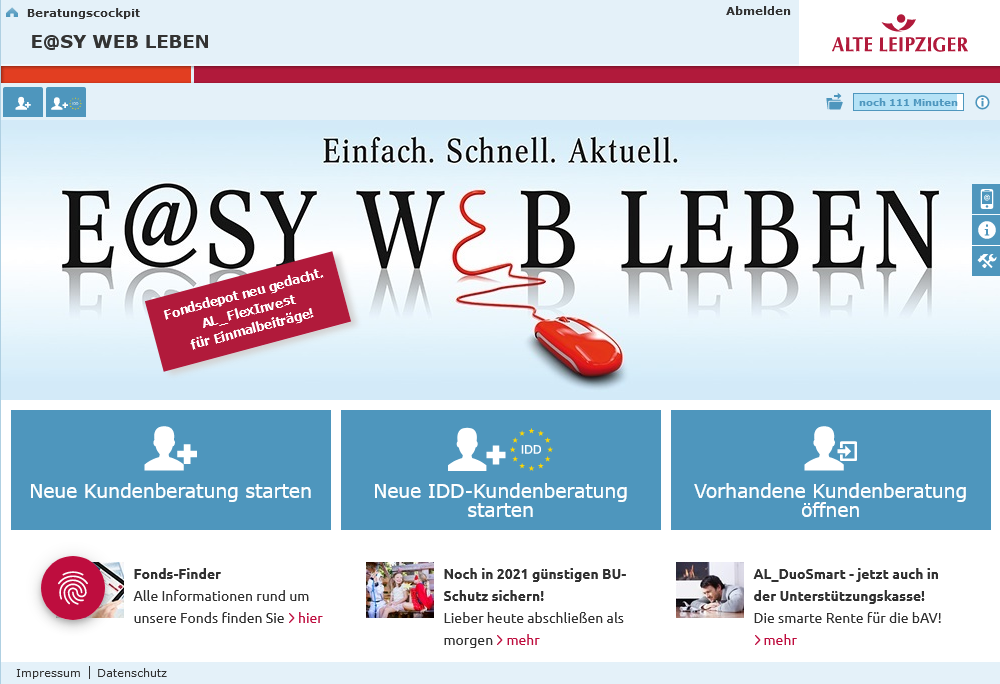
\includegraphics[width=0.8\columnwidth]{images/Easy_Web_Leben_allgemein.png}
\caption{Die Startseite von Easy Web \cite{easy_web}: Es können Kundenprofile zur Kalkulation verschiedener Altersvorsorgeprodukte angelegt und gespeichert werden. Zudem besteht die Möglichkeit ein Kund*innenprofil im Rahmen der IDD-Versicherungsvertriebsrichtlinie anzulegen. Screenshot erstellt am 15.12.2021.}
\label{fig:easyWeballg}
\end{figure}

Verschiedene Konzepte der privaten und betrieblichen Altersvorsorge stehen bei Easy Web zur Auswahl. Mittels einer Registerkarte können Nutzer*innen von Easy Web bei einer Kund*innenberatung zwischen den Bereichen der privaten und betrieblichen Altersvorsorge wechseln. Für beide Bereiche steht zudem eine weitere Registerkarte bereit, die zwischen Rentenprodukten, Berufsunfähigkeitsprodukten und Risikolebensversicherungen unterscheidet. Für jede dieser Registerkarte erscheinen mehrere Tarife, die zur Kalkulation ausgewählt werden können. Der Anwendungsfall dieser Arbeit beschränkt sich auf den Bereich der betrieblichen Altersvorsorge und den Bereich der Renten- beziehungsweise 'Vorsorge'-Produkte. Dies entspricht der Zahlung einer lebenslangen Altersrente, einer einmaligen Kapitalauszahlung oder einer Mischung aus den beiden zuvor genannten Varianten bei Erreichen des vordefinierten Rentenalters. Abbildung \ref{fig:easyWebAuswahl} zeigt das Auswahlmenü für den Fall der bAV.

\begin{figure}[!htb]
\centering
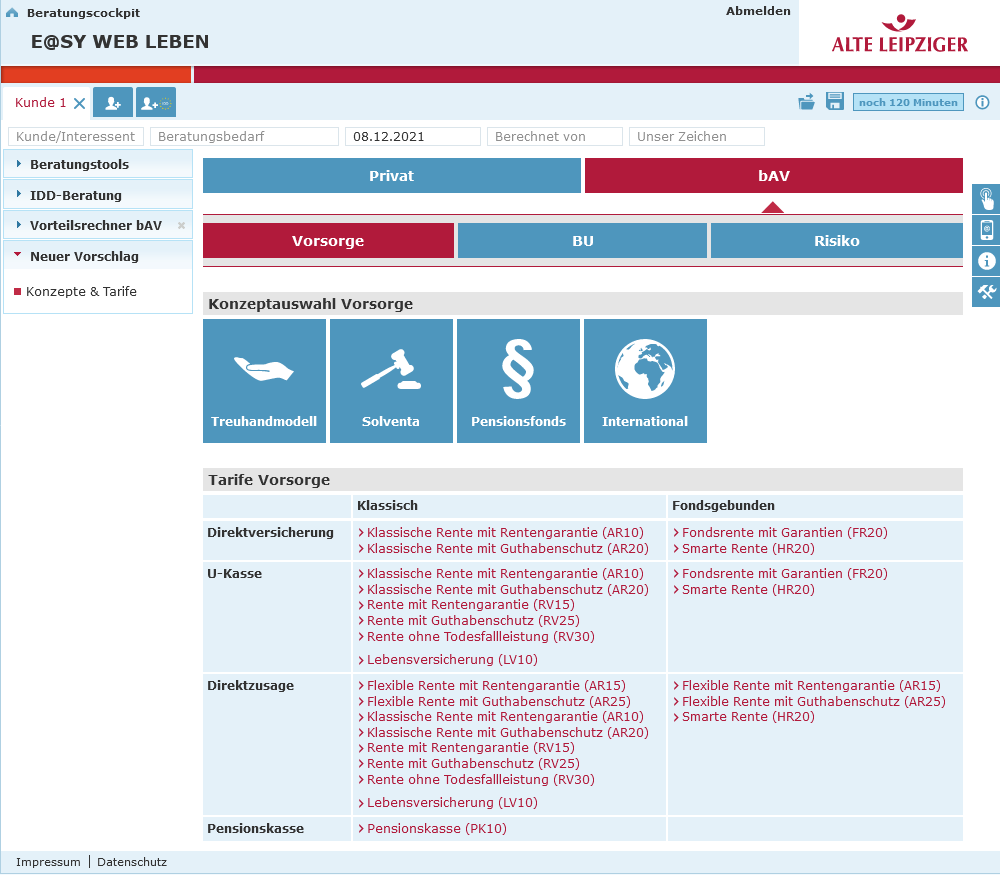
\includegraphics[width=0.7\columnwidth]{images/Easy_Web_Leben_Auswahl.png}
\caption{Das Auswahlmenü von Easy Web bei einer Kund*innenberatung: Es wird zwischen privater und betrieblicher Altersvorsorge unterschieden, zudem können Tarife verschiedener Durchführungswege ausgewählt werden. Screenshot erstellt am 15.12.2021.}
\label{fig:easyWebAuswahl}
\end{figure}

Easy Web ermöglicht die Auswahl von Produkten der bAV über vier der fünf möglichen Durchführungswege (vgl. \autoref{subsec:versicherungsgrundlagen}), die je nach Wahl des Durchführungsweges über eines der verbundenen Unternehmen der ALH-Gruppe abgewickelt werden \cite{alh_bav}. Dabei gilt es zu berücksichtigen, dass Easy Web bzw. die ALH-Gruppe die Durchführungswege intern in einer anderen Art und Weise zuordnet als im allgemeinen Gebrauch: Easy Web unterscheidet im Bereich der Durchführungswege lediglich zwischen Direktversicherung, Pensionskasse und Direktzusage und führt zusätzlich den Parameter 'Art der Rückdeckung' ein. Dieser kann die Werte 'keine', 'Unterstützungskasse' oder 'Rückdeckungsversicherung' annehmen.
\begin{itemize}
\item Direktversicherung / keine Rückdeckung: Abgewickelt über die Alte Leipziger Lebensversicherung a.G.
\item Direktzusage / Unterstützungskasse: Abgewickelt über die Alte Leipziger Unterstützungskasse e.V., rückdeckungsversichert über die Alte Leipziger Lebensversicherung a.G.
\item Direktzusage / Rückdeckungsversicherung: Abgewickelt über die Alte Leipziger Lebensversicherung a.G. als Rückdeckungsversicherung für eine Direktzusage eines Unternehmens.
\item Pensionskasse / keine Rückdeckung: Abgewickelt über die Alte Leipziger Pensionskasse AG
\end{itemize} 

Bei der Wahl der Anlagestrategie der Beiträge der Kundschaft und damit unmittelbar auch der garantierten Leistungen existieren im Bereich der Altersvorsorge die Varianten der klassischen, fondsgebundenen und hybriden Tarife. Bei klassischen Tarifen wird das Guthaben der Kundinnen und Kunden einzig im Deckungskapital des Versicherers angelegt \cite{alh_produkte}. Bei fondsgebundenen Tarifen werden die Beiträge hingegen in Investmentfonds investiert und unterliegen somit den Schwankungen des Kapitalmarktes \cite{alh_produkte}. Hybride Tarife vereinen die beiden Varianten der klassischen und fondsgebundenen Tarife und setzen auf mehrere Töpfe in der Anlage der Beiträge der Kundschaft \cite{alh_produkte}. Im Bereich der bAV vertreibt die ALH-Gruppe keine Produkte mit reiner Fondsanlage, sondern bezeichnet Produkte mit hohem Anteil in der Fondsanlage und zusätzlichen Garantiekomponenten als fondsgebundene Produkte \cite{alh_produkte}. Diese Produkte werden in der Eingabemaske von Easy Web auch als fondsgebunden angezeigt (vgl. Abbildung \ref{fig:easyWebAuswahl}). 

Im folgenden werden die verschiedenen Tarife vorgestellt, welche bei Easy Web ausgewählt werden können. Die Erläuterungen basieren auf \cite{alh_produkte}:
\begin{itemize}
\item Rente mit Rentengarantie (RV15) / mit Guthabenschutz (RV25) / ohne Todesfallleistung (RV30): Als Variante der klassischen Tarife wandern die Beiträge der Versicherten bei diesen Tarifen vollständig in das Deckungskapital der Alten Leipziger Lebensversicherung a. G. und werden zudem mit einem Rechnungszins vollständig garantiert. Zusätzlich bestimmt die Wahl des Tarifs zusätzliche Bausteine im Todesfall des Leistungsempfängers: Bei Wahl der Rentengarantie wird ein bestimmtes Alter der versicherungsnehmenden Person bestimmt oder eine bestimmte Dauer ab Rentenbeginn festgelegt, bis zu welchem die Rente auch im Todesfall an Hinterbliebene weiterhin ausbezahlt wird. Bei Wahl des Guthabenschutzes wird das verbleibende Guthaben nach Abzug der bereits gezahlter Renten an Hinterbliebene ausbezahlt. Die dritte Variante verzichtet auf jegliche Leistungen im Todesfall. Diese drei Tarife können bei Easy Web nur über die Durchführungswege der Direktzusage / Rückdeckungsversicherung oder Direktzusage / Unterstützungskasse ausgewählt werden.
\item Moderne klassische Rente mit Rentengarantie (AR10) / mit Guthabenschutz (AR20): Die Tarife AR10 und AR20 gleichen in ihrer Anlagestruktur der Tarife RV15, RV25 und RV30. Die Beiträge werden im Deckungsstock in sichere Kapitalanlagen investiert und werden für die Rentenbezugszeit garantiert. Die moderne klassische Rente basiert auf einem niedrigeren Garantiezins als die Tarife RV15, RV25 und RV30 und ermöglicht zudem eine flexible Gestaltung der Beitragshöhe. Der Todesfallschutz (mit Guthabenschutz / Rentengarantie) der modernen klassischen Rente gleicht den korrespondierenden Varianten der Tarife RV15 und R25. Die moderne klassische Rente ist in Easy Web über die Durchführungswege Direktversicherung, Direktzusage / Rückdeckungsversicherung und Direktzusage / Unterstützungskasse verfügbar.
\item Pensionskasse (PK10): Dieser Tarif ist der einzige Tarif, der in Easy Web über den Durchführungsweg der Pensionskasse zur Verfügung steht. Er gleicht in seiner Anlagestruktur der modernen klassischen Rente mit Rentengarantie. Im Allgemeinen unterscheiden sich die beiden Tarife PK10 und AR10 kaum, die wesentliche Ausnahme bildet dabei die Abwicklung des Tarifs über die Pensionskasse im Falle des Tarifs PK10 und über die Lebensversicherungsgesellschaft im Falle des Tarifs AR10.
\item Flexible Rente mit Rentengarantie (AR15) / mit Guthabenschutz (AR15): Die flexible Rente der ALH-Gruppe entspricht einem statischen hybriden Tarif. Kundinnen und Kunden können den Anteil des Investments in einen selbst gewählten Investmentfonds individuell spezifizieren. Der verbleibende Anteil der Beiträge wird dann im Deckungsstock angelegt und mit einem Rechnungszins garantiert. Für den Anteil der Anlage im Investmentfonds wird zudem ein Rentenfaktor garantiert. Die Tarifvarianten bezüglich des Todesfallschutzes entsprechen denen der modernen klassischen Rente. Ausgewählt werden kann die flexible Rente in Easy Web nur über den Durchführungsweg Direktzusage / Rückdeckungsversicherung.
\item Fondsrente mit Garantien (FR20): Die Fondsrente mit Garantien ist ebenfalls ein hybrider Tarif, der im Gegensatz zu den Tarifen AR15 und AR25 einem 'dynamischen 3-Topf-Modell' entspricht. Die Anlage der Beiträge setzt sich hier aus dem klassischen Sicherungsvermögen im Deckungsstock des Versicherers, einem Wertsicherungsfonds und einem zusätzlichen individuell gewählten Investmentfonds zusammen. Die Beiträge werden dabei auf die drei verschiedenen Töpfe dynamisch während der Laufzeit aufgeteilt, sodass das Gesamtguthaben eine Verlustobergrenze in vordefinierten Zeiträumen nicht überschreitet. Das Gesamtguthaben der Kundinnen und Kunden wird bis zu einem vordefinierten Grad garantiert. Im Todesfall des Bezugsberechtigten der Rente besitzt der Tarif eine Rentengarantie mit Rentengarantiezeit. Die Fondsrente ist in Easy Web via Direktversicherung und Direktzusage / Unterstützungskasse verfügbar.
\item Smarte Rente (HR20): Die smarte Rente entspricht ebenfalls einem dynamischen hybriden Tarif, der jedoch lediglich auf zwei Anlagetöpfe setzt. Neben der Anlage im Deckungsstock werden die Beiträge lediglich in einen Investmentfonds investiert, der von der ALH-Gruppe vorgeben ist. Zudem unterscheidet sich die smarte Rente gegenüber der Fondsrente derart, dass bei der smarten Rente das Vertragsguthaben vor Rentenbeginn in den Deckungsstock umgeschichtet wird, sodass das garantierte Kapital des Vertrages zu Rentenbeginn sichergestellt ist. Die möglichen Durchführungswege der smarten Rente sind die Direktversicherung, die Unterstützungskasse und die Direktzusage. Auch die smarte Rente besitzt eine Rentengarantie mit Rentengarantiezeit im Todesfall. Wie die moderne klassische Rente kann die smarte Rente bei Easy Web über die Durchführungswege Direktversicherung, Direktzusage / Rückdeckungsversicherung und Direktzusage / Unterstützungskasse ausgewählt werden.
\end{itemize}

Wählt man nun einen der zur Verfügung stehenden Tarife aus, öffnet sich eine Eingabemaske zur Eingabe verschiedener Parameter, welche zur Rentenkalkulation zur Rate gezogen werden. Neben Angaben zur versicherten Person müssen Nutzer*innen von Easy Web zudem Informationen zum gewählten Tarif, eventuellen Zusatzversicherungen und der optionalen Beitragsdynamik angeben. Darüber hinaus werden je nach Wahl des Tarifs und Durchführungsweges detaillierte Angaben zum Versicherungsschutz verlangt: Dies umfasst bei allen Tarifen den Versicherungsbeginn, die Art der Finanzierung, die Höhe des Beitrags, das Renteneintrittsalter und die Periodizität der Beitragszahlungen. Ein weiteres Fenster unter der Bezeichnung 'Details', das jedoch nur bei bestimmten Tarifen angezeigt wird, erlaubt zudem die Angabe zusätzlicher detaillierter Faktoren: So können dort beispielsweise Zuzahlungen zu Beginn des Vertragsabschlusses (bei den Durchführungswegen Direktversicherung, Pensionskasse, Direktzusage) oder die genutzten Freibeträge im Sinne von § 3 Nr. 63 EStG und § 40 b EStG (bei den Durchführungswegen Pensionskasse und Direktversicherung, vgl. \autoref{subsec:versicherungsgrundlagen}) spezifiziert werden. Abbildung \ref{fig:easyWebEingabe} zeigt die Eingabemaske beispielhaft für den Tarif 'Klassische Rente mit Rentengarantie (AR10)' des Durchführungswegs Direktversicherung.

\begin{figure}
\centering
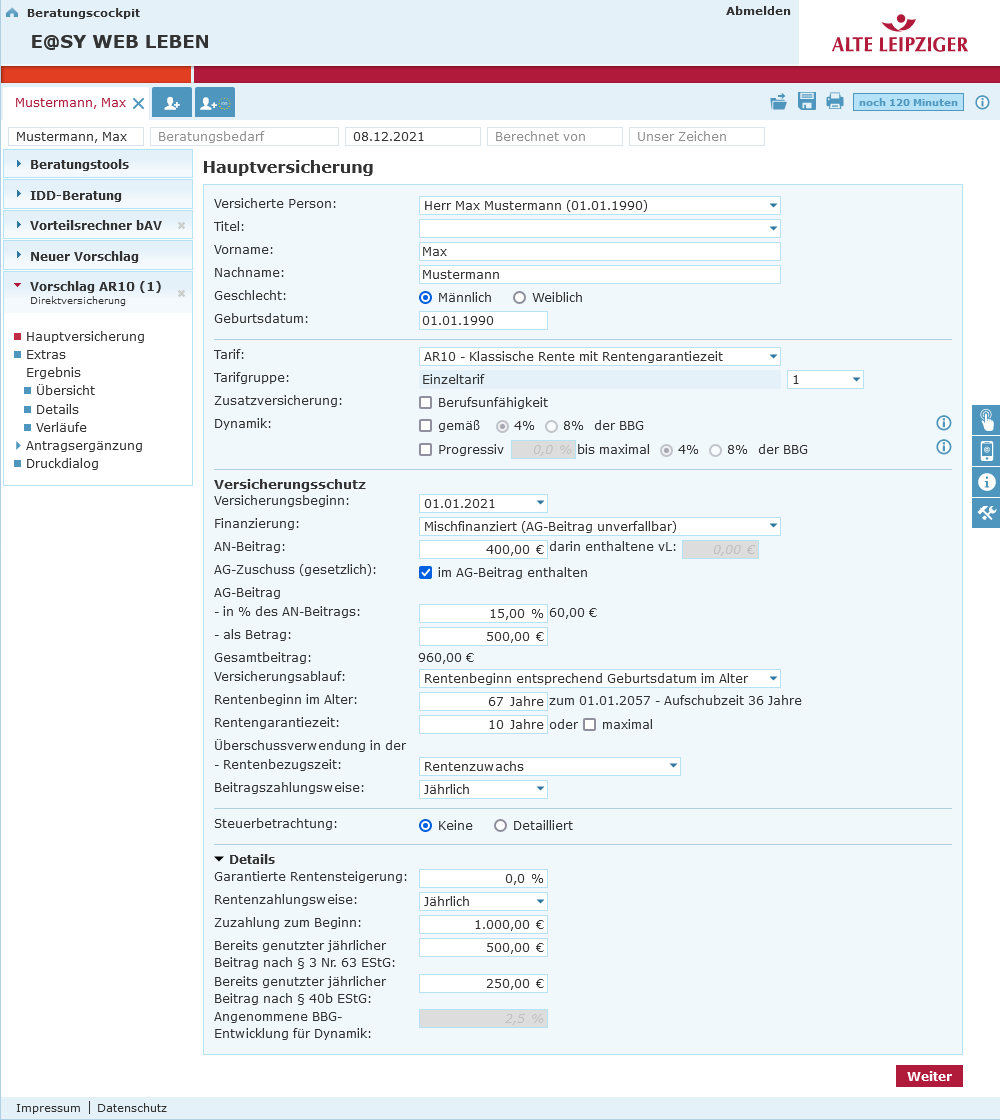
\includegraphics[width=0.72\columnwidth]{images/Easy_Web_Eingabe.png}
\caption{Die Eingabemaske für den Tarif 'Klassische Rente mit Rentengarantie (AR10)' des Durchführungswegs Direktversicherung. Im oberen Bereich werden Angaben zur versicherten Person verlangt, darunter folgt die Spezifizierung der Parameter für den Tarif. Screenshot erstellt am 15.12.2021.}
\label{fig:easyWebEingabe}
\end{figure}

Nach Ausfüllen dieser einführenden Eingabemaske zur Angebotserstellung führt Easy Web Nutzer*innen durch weiterführende Formularfelder: Diese können unter anderem die Spezifizierung der Zusatzversicherungen oder die Wahl der Kapitalanlage bei fondsgebundenen Tarifen sein. Anschließend berechnet Easy Web ein Ergebnis für die garantierte und zu erwartende Rente. 

Fehlerhafte Eingaben werden von Easy Web als solche in den meisten Fällen erst beim Aufruf der Ergebnisseite angezeigt. Dies können einerseits Fehler bezüglich der Kund*innendaten wie ein fehlendes Geburtsdatum sein, andererseits Fehler bezüglich der Werte zum Versicherungsschutz. In beiden Fällen verweist Easy Web auf die Haupteingabemaske zurück und zeigt den konkreten Eingabefehler an. Abbildung \ref{fig:easyWebFehler} zeigt eine beispielhafte Fehlermeldung im Falle einer Eingabe eines jährlichen Beitrags von 0 Euro für den Tarif AR10 und den Durchführungsweg der Direktversicherung.

\begin{figure}[!htb]
\centering
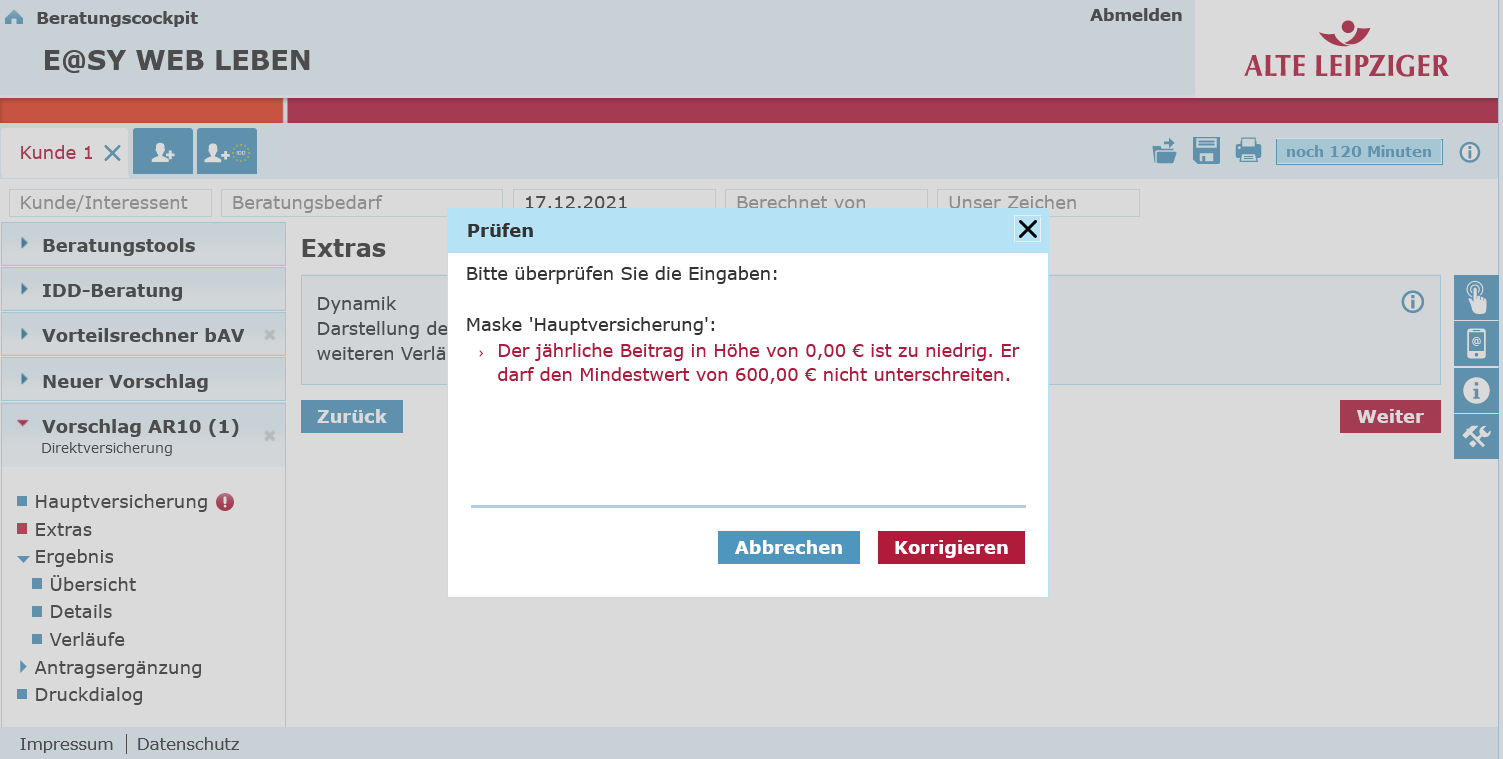
\includegraphics[width=0.8\columnwidth]{images/Easy_Web_Fehler.png}
\caption{Fehlermeldung von Easy Web bei einer Eingabe des Beitrags von 0 Euro im Tarif AR10 des Durchführungswegs Direktversicherung. Screenshot erstellt am 15.12.2021.}
\label{fig:easyWebFehler}
\end{figure}

\section{Implementierung}\label{sec:implementierung}

Im folgenden Abschnitt wird die konkrete Umsetzung zur Beantwortung der Fragestellung dieser Arbeit vorgestellt. Der zugehörige Programmcode kann öffentlich zugänglich auf der Github-Plattform eingesehen werden \cite{github}.

Das im vorausgehenden Abschnitt erwähnte Fehlerverhalten von Easy Web steht dabei im Fokus: Anhand der Methoden des Combinatorial Testing (vgl. \autoref{sec:combinatorialTesting}) werden verschiedene Mengen an Testfällen zur Überprüfung der Plausibilität der möglichen Eingaben in Easy Web erstellt und verglichen. Dies erfolgt anhand mehrerer Ansätze, die unterschiedliche Teilfragestellungen beantworten:
\begin{enumerate}
\item Erstellung eines 'Basis-Systems' mit Combinatorial Testing unter Berücksichtigung von Bedingungen des zu testenden Systems: Ist es überhaupt möglich Testfälle für ein System wie Easy Web mittels Combinatorial Testing zu erstellen?
\item Vergleich Combinatorial Testing / Random Testing: Schafft Combinatorial Testing Vorteile gegenüber einem zufälligen Testverfahren?
\item Erweiterung des 'Basis-Systems' zu einem 'Erweiterten System': Inwieweit verändert die Einführung komplexerer Parameterstrukturen -- im Speziellen die Einführung der Finanzierungsart und separate Parameter für Arbeitgeber- und Arbeitnehmerbeitrag -- die Resultate im Vergleich zum einfacheren 'Basis-System'?
\item $t$-fache Kombinatorik für jeden Durchführungsweg: Ist es sinnvoll spezifische Parameter zu extrahieren -- im Speziellen die Kombinationen der Durchführungswege und der Art der Rückdeckung -- und für deren Werte jeweils unabhängig voneinander Testmengen mittels Combinatorial Testing zu erstellen?
\item Vergleich verschiedener Combinatorial Testing Tools / Algorithmen: Welcher Algorithmus beziehungsweise welches Tool ist für die praktische Anwendung am nützlichsten?
\end{enumerate}

Als Grundlage aller Untersuchungen dienen die Vorsorge-Tarife der bAV in Easy Web, wie sie in Abbildung \ref{fig:easyWebAuswahl} zu erkennen sind. Der Tarif der Lebensversicherung (LV10) wird im Anwendungsfall nicht berücksichtigt. 

Der Anwendungsfall bezieht sich aus Gründen der Übersichtlichkeit auf eine reduzierte Auswahl der möglichen Eingabeparameter der verschiedenen Tarife in der Eingabemaske von Easy Web (vgl. \autoref{fig:easyWebEingabe}): Angaben zur versicherten Person werden im Rahmen dieser Arbeit fest vorgegeben und sind nicht variabel, ebenso Parameter optionaler Zusatzversicherungen \footnote{Verwendete Ausprägungen der Parameter zur versicherten Person und optionaler Zusatzversicherung: Max Mustermann, männlich, geb. 01.01.1980, keine Zusatzversicherung, keine Dynamik}. Außerdem werden eine progressive Beitragsentwicklung und jegliche Parameter zur Rentenauszahlung wie Rentenbeginn oder etwaige Todesfallleistungen ausgeschlossen. Letztere Annahme führt dazu, dass für die Tarife AR10 / AR20, AR15 / AR25, RV15 / RV25 / RV30 im Rahmen dieser Arbeit jeweils keine Unterschiede existieren und diese deshalb im Sinne einer Äquivalenzklassenbildung (vgl. \autoref{subsub:äquivalenklassenmethode}) zusammengefasst werden: AR10 / AR20 wird im Folgenden als AREven bezeichnet, AR15 / AR25 als AROdd und RV15 / RV25 / RV30 als RVx. 

Weitere Annahmen an das im Anwendungsfall untersuchte System sind: Die Beitragszahlung zur bAV erfolgt jährlich mit einem beliebigen, aber festen Beitrag. Dabei wird angenommen, dass die Arbeitgeberzulage stets 0\% beträgt. Der Versicherungsbeginn wird auf den 01.01.2021 festgesetzt, der Rentenbeginn soll stets am 01.01. eines Jahres erfolgen. Dies bewirkt, dass das Versicherungsjahr dem Kalenderjahr entspricht und infolgedessen alle Beitragsgrößen sich auf das Kalenderjahr beziehen.


\subsection{Basis-System}\label{subsec:ImplBasisModell}

Aus den getroffenen Annahmen ergibt sich ein zu testendes System aus verschiedenen Parametern, welches als Grundlage der Untersuchungen dieser Arbeit dient. Dieses Testsystem wird im Folgenden als 'Basis-System' bezeichnet. Das Basis-System umfasst sieben verschiedene Parameter und 25 Bedingungen, die berücksichtigt werden müssen. Die Bedingungen umfassen Tarifvarianten in Abhängigkeit des Durchführungswegs und der Art der Rückdeckung und Vorgaben in Bezug auf die Wahl der möglichen Werte für die verschiedenen Parameter. Konkrete Beispiele werden dazu in den folgenden Absätzen aufgeführt, zudem kann die vollständige Liste der Bedingungen im Anhang dieser Arbeit nachgelesen werden (vgl. \autoref{sec:bedingungenSimple}). \autoref{tab:sutSimple} zeigt einen Überblick über die verschiedenen Parameter des Basis-Systems und die zugehörigen möglichen Werte.

\begin{table}[htb!]
\footnotesize
\begin{tabularx}{\textwidth}{|X|l|}
\hline
\cellcolor{grauinfo}Parameter                                      & \cellcolor{grauinfo}Mögliche Werte                                       \\ \hline
Durchführungsweg                               & Direktversicherung, Direktzusage, Pensionskasse      \\ \hline
Art der Rückdeckung\footnotemark               & keine, Rückdeckungsversicherung, Unterstützungskasse \\ \hline
Tarif                                          & AREven, AROdd, FR20, HR20, PK10, RVx                 \\ \hline
Beitrag                                        & 0, 24, 299, 599, 600, 5.000, 125.001                 \\ \hline
Zuzahlung zu Beginn                            & 0, 99, 299, 2.000, 5.001, 1.000.001                  \\ \hline
Bereits genutzter Beitrag nach § 40 b EStG     & 0, 2.148, 2.149                                      \\ \hline
Bereits genutzter Beitrag nach § 3 Nr. 63 EStG & 0, 2.068, 4.068                                      \\ \hline
\end{tabularx}
\normalsize
\caption{Die Parameter und möglichen Werte des Basis-Systems}
\label{tab:sutSimple}
\end{table}
\footnotetext{Die Ausprägung der Unterstützungskasse wird in der Literatur üblicherweise als eigener Durchführungsweg betrachtet (vgl. dazu \autoref{subsec:versicherungsgrundlagen}). Easy Web ordnet die Unterstützungskasse intern dem Durchführungsweg Direktzusage zu und führt sie als mögliche Art der Rückdeckung.} 

Das Basis-System unterscheidet nicht zwischen den verschiedenen Finanzierungsarten der bAV: Als Vereinfachung wird angenommen, dass nur ein einziger Wert als Beitragshöhe existiert. Dies bedeutet im Konkreten: Falls die modellierte Rente Arbeitgeber-finanziert / Arbeitnehmer-finanziert ist, fällt der gewählte Beitrag vollständig dem Arbeitgeber / dem Arbeitnehmer zu. Falls die Rente Misch-finanziert ist, soll der Beitrag zur Hälfte auf beide Parteien aufgeteilt werden. Eine detaillierte Betrachtungsweise der Finanzierungsart wird im Erweiterten System (vgl. \autoref{subsec:ImplErweitertesModell}) aufgegriffen, wobei ebenfalls stets absolute Beiträge als Basis dienen. Im Kontext der Misch-Finanzierung werden daher relative Arbeitgeber-Anteile ausgeschlossen.

Für die Parameter Durchführungsweg, Art der Rückdeckung und Tarif entsprechen die möglichen Werte des Basis-System den Auswahlmöglichkeiten des Auswahlmenüs im Bereich 'Vorsorge' der bAV bei Easy Web (vgl. \autoref{fig:easyWebAuswahl}). Einzige Ausnahme: Der Tarif LV10 wird ausgeschlossen.

Die möglichen Werte für Beitragshöhe, Zuzahlung zu Beginn, Bereits genutzter Beitrag nach § 40 b EStG und Bereits genutzter Beitrag nach § 3 Nr. 63 EStG ergeben sich aus einer Analyse des Fehlerverhaltens von Easy Web. Durch wiederholte Experimente bei der Nutzung von Easy Web und einer Analyse der Produktinformationen \cite{alh_produkte} wurden untere und obere Schranken für die Höhe der Beiträge ermittelt, die Easy Web als Fehlergrenzen betrachtet. \autoref{tab:beitragsgrenzen} zeigt die Auflistung der Beitragsgrenzen in Abhängigkeit des Durchführungswegs, der Art der Rückdeckung und der zugehörigen Tarife. In roter Farbe sind die unteren Schranken aufgeführt, in grüner Farbe die oberen Schranken.

% Please add the following required packages to your document preamble:
% \usepackage{multirow}
% \usepackage{graphicx}
% Please add the following required packages to your document preamble:
% \usepackage{multirow}


% Please add the following required packages to your document preamble:
% \usepackage{multirow}


% Please add the following required packages to your document preamble:
% \usepackage{multirow}
% Please add the following required packages to your document preamble:
% \usepackage{multirow}


\renewcommand{\arraystretch}{2.5}

\begin{table}[!htb]
\scriptsize
\begin{tabular}{|M{\durchfuehrungsweg}|M{\finanzierung}|M{\tarife}|M{\beitrag}|M{\zuzahlung}|M{\bvierzig}|M{\bdreiEStG}|}
\hline
\cellcolor{grauinfo}Durchführungs- weg / Art der Rückdeckung &
  \cellcolor{grauinfo}Finanz- ierung &
  \cellcolor{grauinfo}Tarife &
  \cellcolor{grauinfo}Beitrag &
  \cellcolor{grauinfo}Zuzahlung &
  \cellcolor{grauinfo}Verw. Beitrag § 40 b &
  \cellcolor{grauinfo}Verw. Beitrag § 3(63) \\ \hline
\multirow{2}{=}{\centering Direkt- versicherung / keine} &
  \multirow{2}{=}{\centering \textit{AN, AG, Misch}} &
  \multirow{2}{=}{\centering AREven, HR20, FR20} &
  \multicolumn{1}{M{\beitrag}|}{\textcolor{red2}{$\geq$ 600}} &
  \multicolumn{1}{M{\zuzahlung}|}{\textcolor{red2}{= 0 bzw. $\geq$ 100}} &
  \multicolumn{2}{M{\bZwei}|}{\textcolor{red2}{$\geq$ 0}} \\ \cline{4-7} 
 &
   &
   &
  \multicolumn{4}{M{\bAlle}|}{\textcolor{modGreen}{Summe aller Beiträge $\leq$ 6.816   (BBG-Grenze) \& Beitrag 40b $\leq$ 2.148}} \\ \hline


\multirow{2}{=}{\centering Pensionskasse / keine} &
  \multirow{2}{=}{\centering \textit{AN, AG, Misch}} &
  \multirow{2}{=}{\centering PK10} &
  \multicolumn{1}{M{\beitrag}|}{\textcolor{red2}{$\geq$ 300}} &
  \multicolumn{1}{M{\zuzahlung}|}{\textcolor{red2}{= 0 bzw. $\geq$ 300}} &
  \multicolumn{2}{M{\bZwei}|}{\textcolor{red2}{$\geq$ 0}} \\ \cline{4-7} 
 &
   &
   &
  \multicolumn{4}{M{\bAlle}|}{\textcolor{modGreen}{Summe aller Beiträge $\leq$ 6.816   (BBG-Grenze) \& Beitrag 40b $\leq$ 2.148}} \\ \hline

\multirow{6}{=}{\centering Direktzusage / Unterstütz- ungskasse} &
  \multirow{6}{=}{\centering \textit{AN, AG}} &

  \multirow{2}{=}{\centering AREven, HR20} &
  \multicolumn{1}{M{\beitrag}|}{\textcolor{red2}{$\geq$ 600}} &
  \multicolumn{3}{M{\bDrei}|}{\multirow{6}{=}{\centering \vspace{-1cm}\hspace{-0.8cm}--}} \\ \cline{4-4}
 &
   &
   &
  \multicolumn{1}{M{\beitrag}|}{\textcolor{modGreen}{$\leq$ 125.000 (Verweis auf Direktionsanfrage)}} &
  \multicolumn{3}{l|}{} \\ \cline{3-4} 
  &
  &
\multirow{2}{=}{\centering FR20} &
  \multicolumn{1}{M{\beitrag}|}{\textcolor{red2}{$\geq$ 300}} &
  \multicolumn{3}{l|}{} \\ \cline{4-4}
&
&
&
  \multicolumn{1}{M{\beitrag}|}{\textcolor{modGreen}{$\leq$ 125.000 (Verweis auf Direktionsanfrage)}} &
  \multicolumn{3}{l|}{} \\ \cline{3-4} 
&
&
\multirow{2}{=}{\centering RVx} &
  \multicolumn{1}{M{\beitrag}|}{\textcolor{red2}{$\geq$ 25 \& wie bei Rückdeckungsversicherung / RVx}} &
  \multicolumn{3}{l|}{} \\ \cline{4-4}
&
&
&
  \multicolumn{1}{M{\beitrag}|}{\textcolor{modGreen}{$\leq$ 125.000 (Verweis auf Direktionsanfrage)}} &
  \multicolumn{3}{l|}{} \\ \hline

%%

\multirow{4}{=}{\centering Direktzusage / Rückdeckungs- versicherung} &
  \multirow{4}{=}{\centering \textit{AG}} &
  \multirow{2}{=}{\centering AREven, AROdd,   HR20} &
  \multicolumn{1}{M{\beitrag}|}{\textcolor{red2}{$\geq$ 600}} &
  \multicolumn{1}{M{\zuzahlung}|}{\textcolor{red2}{$\geq$ 0}} &
  \multicolumn{2}{M{\bZwei}|}{\multirow{4}{=}{\centering  \vspace{-0.5cm}\hspace{-0.4cm}--}} \\ \cline{4-5}
 &
   &
   &
  \multicolumn{1}{M{\beitrag}|}{\textcolor{modGreen}{$\leq$   125.000 (Verweis auf Direktionsanfrage)}} &
  \multicolumn{1}{M{\zuzahlung}|}{\textcolor{modGreen}{$\leq$ 1 Mio.}} &
  \multicolumn{2}{l|}{} \\ \cline{3-5}
 &
   &
  \multirow{2}{=}{\centering RVx} &
  \multicolumn{1}{M{\beitrag}|}{\textcolor{red2}{Ergibt sich aus garantierter Rente von 600 Euro (hängt vom Alter ab)}} &
  \multicolumn{1}{M{\zuzahlung}|}{\textcolor{red2}{= 0 bzw. $\geq$ 500}} &
  \multicolumn{2}{l|}{} \\ \cline{4-5}
 &
   &
   &
  \multicolumn{1}{M{\beitrag}|}{\textcolor{modGreen}{$\leq$   125.000 (Verweis auf Direktionsanfrage)}} &
  \multicolumn{1}{M{\zuzahlung}|}{\textcolor{modGreen}{$\leq$ 5.000}} &
  \multicolumn{2}{l|}{} \\ \hline


\end{tabular}

\normalsize
\caption{Grenzen (in Euro) der möglichen Eingabewerte der Beitragsparameter in Easy Web in Abhängigkeit des Durchführungswegs, der Rückdeckung und der jeweiligen Tarife. Rot sind untere Schranken markiert, grün obere Schranken}
\label{tab:beitragsgrenzen}
\end{table}

\renewcommand{\arraystretch}{1.5}

Für die Durchführungswege Direktversicherung und Pensionskasse ergibt sich eine kombinierte oberere Schranke für Beitragshöhe, Zuzahlung zu Beginn, Bereits genutzter Beitrag nach § 40 b EStG und Bereits genutzter Beitrag nach § 3 Nr. 63 EStG: Die Summe dieser Parameter darf den Wert der 8\%-Fördergrenze der Beitragsbemessungsgrenze nach § 3 Nr. 63 EStG nicht überschreiten (vgl. \autoref{subsec:versicherungsgrundlagen}). Höhere Beiträge als der Wert von 6.816 Euro erlaubt Easy Web bei der Eingabe nicht. Darüber hinaus darf bei den Durchführungswegen Direktversicherung und Pensionskasse der genutzte Beitrag im Sinne von § 40 b EStG den Maximalbetrag von 2.148 Euro nicht überschreiten (vgl. \autoref{subsec:versicherungsgrundlagen}).

Für die Höhe des Beitrages existiert beim Durchführungsweg der Direktzusage eine obere Schranke, die durch den jährlichen Maximalbeitrag von 125.000 Euro festgesetzt ist. Falls dieser Wert überschritten wird, berechnet Easy Web keine Rente und zeigt eine Fehlermeldung mit einem Verweis auf eine notwendige Direktionsanfrage an. Für die untere Schranke gilt für die Tarife der klassischen RVx-Rente eine besondere Regelung: Die Untergrenze ergibt sich dabei aus einer garantierten jährlichen Rente von 600 Euro, die sich über die Faktoren der Beitragshöhe und der Dauer der Beitragszahlungen (beziehungsweise dem Alter der versicherten Person) ermitteln lässt.

Die bereits genutzten Beiträge nach § 40 b EStG nach § 3 Nr. 63 EStG spielen aufgrund der gesetzlichen Regelungen nur für die Durchführungswege Direktversicherung und Pensionskasse eine Rolle, eine Zuzahlung ermöglicht Easy Web lediglich beim Durchführungsweg Direktzusage und der Rückdeckung via Rückdeckungsversicherung. In diesen Fällen wird durch Bedingungen an das zu testende System der Wert 0 für die ausgeschlossenen Parameter festgesetzt. So gilt als Beispiel für die Kombination Direktzusage / Rückdeckungsversicherung: \textit{Durchführungsweg = 'Direktzusage' \&\& Art der Rückdeckung = 'Rückdeckungsversicherung' $\Rightarrow$ Verw. Beitrag § 40 b = 0 \&\& Verw. Beitrag § 3(63) = 0.}

Darüber hinaus setzt Easy Web in bestimmten Fällen eine Mindestanforderung an die Höhe der Zuzahlung voraus: Die Zuzahlung bei den Kombinationen Direktversicherung / keine Rückdeckung, Pensionskasse / keine Rückdeckung und Direktzusage / Rückdeckungsversicherung / RVx muss entweder gleich 0 sein oder einen Mindestbetrag überschreiten (vgl. \autoref{tab:beitragsgrenzen}).

\hspace{1cm}Die konkreten Werte für Beitragshöhe, Zuzahlung zu Beginn, Bereits genutzter Beitrag nach § 40 b EStG und Bereits genutzter Beitrag nach § 3 Nr. 63 EStG wurden anhand der Analyse aus \autoref{tab:beitragsgrenzen} und den Methoden der Äquivalenzklassenbildung (vgl. \autoref{subsub:äquivalenklassenmethode}) und Grenzwertanalyse (vgl. \autoref{subsub:grenzwertanalyse}) ermittelt. Für jede Schranke des Systems wurden Äquivalenzklassen oberhalb und unterhalb der Schranke angenommen und darauf aufbauend mindestens ein Wert pro Klasse in das Testsystem aufgenommen. Dies gilt insbesondere auch für kombinierte Schranken mehrerer Parameter wie die 8\%-Fördergrenze der Beitragsbemessungsgrenze nach § 3 Nr. 63 EStG. Zudem wurden im Besonderen die Grenzwerte im Sinne der Grenzwertanalyse betrachtet, sodass pro Äquivalenzklasse die betroffenen Schranken möglichst exakt getroffen werden. Beispiel hierfür sind die Werte 2.148 Euro und 2.149 Euro für den bereits genutzten Beitrag nach § 40 b EStG. 

Die aus diesem Vorgehen resultierenden Werte für die verschiedenen Beitragsparameter sind in \autoref{tab:äquivalenzklassenSimple} dargestellt. Dabei gilt es zu berücksichtigen, dass nicht alle Werte der Beitragsparameter, die in \autoref{tab:sutSimple} aufgeführt sind, für alle Durchführungswege relevant sind: Durch zusätzliche Bedingungen an das Testsystem werden bei der Erstellung der Testmengen lediglich die in \autoref{tab:äquivalenzklassenSimple} aufgeführten Werte für die Kombinationen der Durchführungswege, Art der Rückdeckung und Tarife bei der Erstellung der Testfälle berücksichtigt. Beispielsweise gilt für die Kombination Direktversicherung / keine Rückdeckung bei allen Tarifen folgende Bedingung: \textit{Durchführungsweg = 'Direktversicherung' $\Rightarrow$ Beitrag = 0 || Beitrag = 599 || Beitrag = 600.}


\renewcommand{\arraystretch}{2.5}

\begin{table}[htb!]
\scriptsize
\begin{tabular}{|M{\durchfuehrungsweg}|M{\durchfuehrungsweg}|M{\zuzahlung}|M{\zuzahlung}|M{\zuzahlung}|M{\zuzahlung}|}
\hline
\cellcolor{grauinfo}Durchführ- ungsweg / Art der Rückdeckung &
  \cellcolor{grauinfo}Tarife &
  \cellcolor{grauinfo}Beitrag &
  \cellcolor{grauinfo}Zuzahlung &
  \cellcolor{grauinfo}Verw. Beitrag §~40~b &
  \cellcolor{grauinfo}Verw. Beitrag §~3~\#63 \\ \hline
  Direktversicherung &
  AREven,   HR20, FR20 &
  0,   599, 600 &
  0,   99, 2.000 &
  0,   2.148, 2.149 &
  0,   2.068, 4.068  \\ \hline

	Pensionskasse &
	 PK10 &
	  0,   299, 599, 600 &
	  0,   299, 2.000 &
	  0,   2.148, 2.149 &
	  0,   2.068, 4.068  \\ \hline

\multirow{3}{=}{\centering Direktzusage / Unterstütz- ungskasse} &
  AREven,   HR20 &
  0,   599, 600, 125.001 &
  \multicolumn{3}{M{\bDrei}|}{\multirow{3}{=}{\centering  \vspace{-0.7cm}\hspace{-1.4cm}--}} \\ \cline{2-3}

   &
  FR20 &
  0,   299, 600, 125.001 &
  \multicolumn{3}{l|}{} \\ \cline{2-3}

   &
  RVx &
  0,   24, 299, 600, 125.001 &
  \multicolumn{3}{l|}{} \\ \hline

%%

\multirow{2}{=}{\centering Direktzusage / Rückdeckungs- versicherung} &
  AREven, AROdd,   HR20 &
  0, 599, 600, 125.001 &
  0, 2.000, 1.000.001 &
  \multicolumn{2}{M{\bZwei}|}{\multirow{2}{=}{\centering  \vspace{-0.7cm}\hspace{-1.4cm}--}} \\ \cline{2-4}

   &
  RVx &
  0,   24, 299, 5.000, 125.001 &
  0, 299, 2.000, 5.001 &
  \multicolumn{2}{l|}{} \\ \hline


\end{tabular}

\normalsize
\caption{Mögliche Werte für die verschiedenen Beitragsparameter für das Basis-System in Abhängigkeit des Durchführungswegs, der Art der Rückdeckung und des Tarifs.}
\label{tab:äquivalenzklassenSimple}
\end{table}

\renewcommand{\arraystretch}{1.5}

Das vorgestellte Basis-System dient als Grundlage zur Erstellung einer Menge an Testfälle im Sinne von Combinatorial Testing (vgl. \autoref{sec:combinatorialTesting}). Für die Beantwortung der grundsätzlichen Fragestellung dieser Arbeit wurden Testmengen mit einem Interaktionsparameter von $t = 2$ bis $t = 6$ via ACTS (vgl. \autoref{subsub:acts}) und dem allgemeinen IPOG-Algorithmus (vgl. \autoref{subsub:ipog}) erstellt.


\subsection{Vergleich Combinatorial Testing / Random Testing}\label{subsec:ImplRandomTesting}

Die grundlegende Fragestellung, die durch Erstellung von Testmengen des Basis-Systems beantwortet wird, sollte im Weiteren durch einen Vergleich mit einer naiven, zufallsbasierten Herangehensweise erweitert werden und aufzeigen, inwieweit ein systematisches Vorgehen bei der Erstellung von Testmengen hilfreich sein kann. 

Dafür wurde ein Random Testing-Ansatz (vgl. \autoref{subsec:beispieleTests}) für das zuvor vorgestellte Basis-System implementiert: Für eine vordefinierte Anzahl $N$ an Testfällen erzeugt der implementierte Random-Testing-Algorithmus zufällige Testfälle, indem für jeden Parameter des Basis-Systems zufällig ein Wert ausgewählt wird. Der erzeugte Testfall wird dann auf Konsistenz mit den 25 Bedingungen des Basis-Systems geprüft: Falls jener Testfall die Bedingungen des Basis-Systems nicht erfüllt, wird dieser verworfen und ein neuer zufälliger Testfall erstellt. Darüber hinaus prüft der Algorithmus die Testfälle auf Duplikate und verwirft diese im Falle eines bereits existierenden Testfalls.

Als Vergleichsgrößen zum Ansatz des Combinatorial Testing dienen unter anderem Effizienzmetriken des Random Testing-Ansatzes wie die Ausführungszeit und die Anzahl der benötigten Iterationen, die zur Erstellung von $N$ Testfällen benötigt werden. In Bezug auf die Ausführungszeit gilt bei allen Untersuchungen dieser Arbeit, dass diese unter identischen Bedingungen auf derselben Maschine durchgeführt wurden. 

Als weitere Vergleichsgrößen des Random Testings wurden die Abdeckung im Sinne von Combinatorial Testing mit den Metriken der $t$-fachen-Abdeckung (vgl. \autoref{subsub:TAbdeckung}), der Variablen-Wert-Abdeckung (vgl. \autoref{subsub:variablenWert}) und der (0,75-$t$)-Vollständigkeit (vgl. \autoref{subsub:pTVollständigkeit}) geprüft für $t \in \{2,3\}$. Das Random Testing-Verfahren wurde für $N \in \{50, 100, 200, 300\}$ mit jeweils 20 Wiederholungen durchgeführt. Die Ergebnisse wurden schließlich als Mittelwert der 20 Wiederholungen berechnet.


\subsection{Erweitertes System}\label{subsec:ImplErweitertesModell}

Das Basis-System beinhaltet keine spezifische Betrachtungsweise der Finanzierungsart und einer damit verbundenen Trennung zwischen Arbeitgeber- und Arbeitnehmer-Beitrag. Das 'Erweiterte System' greift diesen Aspekt auf und soll aufzeigen, inwiefern sich die Erstellung von Testmengen via Combinatorial Testing auf komplexere Systeme skalieren lässt.

Das Erweiterte System ergänzt das Basis-System durch die Parameter Finanzierungsart (Arbeitgeber-, Arbeitnehmer-, Misch-finanziert) und Arbeitnehmer- und Arbeitgeberbeitrag, der Parameter Beitrag des Basis-Systems entfällt. Das Erweiterte System besitzt folglich neun verschiedene Parameter und zusätzliche sieben Bedingungen an das Testsystem im Vergleich zum Basis-System: Neu hinzugefügte Bedingungen umfassen unter anderem bestimmte Kombinationen aus Durchführungsweg und Art der Rückdeckung, die spezifische Finanzierungsarten voraussetzen. Beispielsweise wird bei Easy Web die Kombination Direktzusage / Rückdeckungsversicherung nur als Arbeitgeber-finanzierte Variante durchgeführt. Die resultierende Bedingung lautet:\textit{ Durchführungsweg = 'Direktzusage' \&\& Art der Rückdeckung = 'Rückdeckungsversicherung' $\Rightarrow$ Finanzierungsart = 'AG-finanziert'}. Die verschiedenen Finanzierungsmöglichkeiten abhängig vom Durchführungsweg, Art der Rückdeckung und Tarif können \autoref{tab:beitragsgrenzen} entnommen werden. \autoref{tab:sutComplex} zeigt eine Übersicht über die Parameter und möglichen Werte des Erweiterten Systems.

\begin{table}[htb!]
\footnotesize
\begin{tabularx}{\textwidth}{|X|l|}
\hline
\cellcolor{grauinfo}Parameter                                      & \cellcolor{grauinfo}Mögliche Werte                                       \\ \hline
Durchführungsweg                               & Direktversicherung, Direktzusage, Pensionskasse      \\ \hline
Art der Rückdeckung                            & keine, Rückdeckungsversicherung, Unterstützungskasse \\ \hline
Tarif                                          & AREven, AROdd, FR20, HR20, PK10, RVx                 \\ \hline
\textbf{Finanzierung}								   &AG-finanziert, AN-finanziert, Misch-finanziert     \\ \hline
\textbf{AN-Beitrag}                                    & 0, 299, 599, 600, 1.500, 125.001                     \\ \hline
\textbf{AG-Beitrag }                                    & 0, 24, 299, 599, 600, 1.500, 125.001                   \\ \hline
Zuzahlung zu Beginn                            & 0, 99, 299, 2.000, 5.001, 1.000.001                  \\ \hline
Bereits genutzter Beitrag nach § 40 b EStG     & 0, 2.148, 2.149                                      \\ \hline
Bereits genutzter Beitrag nach § 3 Nr. 63 EStG & 0, 2.068, 4.068                                      \\ \hline
\end{tabularx}
\normalsize
\caption{Die Parameter und möglichen Werte des Erweiterten Systems: Das Erweiterte System umfasst zusätzliche Parameter bezüglich der Finanzierungsart und der Unterscheidung in Arbeitgeber- und Arbeitnehmerbeitrag}.
\label{tab:sutComplex}
\end{table}

Analog zur Ermittlung der Werte der Parameter Beitragshöhe, Zuzahlung zu Beginn, Bereits genutzter Beitrag nach § 40 b EStG und Bereits genutzter Beitrag nach § 3 Nr. 63 EStG im Basis-System wurden die Werte für die verschiedenen Parameter des Erweiterte Systems auf Basis der Beitragsgrenzen in \autoref{tab:beitragsgrenzen} festgesetzt. Dabei wurden wie beim Basis-System die Methoden der Äquivalenzklassenmethode (vgl. \autoref{subsub:äquivalenklassenmethode}) und Grenzwertanalyse (vgl. \autoref{subsub:äquivalenklassenmethode}) kombiniert. Eine Übersicht über die möglichen Werte der verschiedenen Parameter des Erweiterten Systems (\autoref{tab:äquivalenzklassenComplex}) und die Bedingungen des Erweiterten Systems (\autoref{sec:bedingungenComplex}) befindet sich im Anhang dieser Arbeit.

Das Erweiterte System wurde mit dem Basis-System in Bezug auf die Anzahl der erzeugten Testfälle für die Interaktionsparameter $t \in \{2,3,4,5,6\}$ verglichen, ebenfalls unter Anwendung des allgemeinen IPOG-Algorithmus (vgl. \autoref{subsub:ipog}) via ACTS (vgl. \autoref{subsub:acts}): Dabei wurde zudem untersucht, wie sich das Laufzeitverhalten durch die zusätzlichen Parameter verändert.

\subsection{$t$-fache Kombinatorik für jeden Durchführungsweg}\label{subsec:ImplFullCombinations}

Sowohl beim Basis-System als auch beim Erweiterten System sind die Parameter Durchführungsweg und Art der Rückdeckung Teil der Kombinatorik bei der Erstellung der Testfallmengen mit $t$-facher Abdeckung. Dabei kann es jedoch passieren, dass durch die Reduktion der Kombinatorik auf den Wert $t$ erwünschte Kombinationen verschiedener Parameter unberücksichtigt bleiben. \autoref{tab:erklärungFullCombination} verdeutlicht dieses Prinzip: Sei $t=2$ gegeben, dann erfüllt ein Testfall mit Tarif = 'AREven' und Beitrag = '600' bereits die notwendige 2-fach-Abdeckung für das Parameterpaar Tarif / Beitrag. In \autoref{tab:erklärungFullCombination} entspricht dies dem ersten Eintrag mit Durchführungsweg Direktversicherung ohne Rückdeckung.

\renewcommand{\arraystretch}{2}
\begin{table}[!htb]
\footnotesize
\begin{tabular}{|M{\tabOther}|M{\tabOther}|M{\tabBeitrag}|M{\tabBeitrag}|}
\hline
\cellcolor{grauinfo}Durchführungsweg & \cellcolor{grauinfo}Art der Rückdeckung & \cellcolor{grauinfo}Tarif & \cellcolor{grauinfo}Beitrag \\ \hline
Direktversicherung      & keine                     & AREven   & 600   \\ \hline
Direktzusage       & Unterstützungs- kasse & AREven    & 599    \\ \hline
Direktzusage       & Rückdeckungs- versicherung & AREven    & 125.001     \\ \hline
\end{tabular}
\normalsize
\caption{Entstehende Problematik bei Einbezug des Durchführungswegs und der Art der Rückdeckung in die $t$-fach-Kombinatorik bei der Erstellung von Testmengen: Für $t=2$ wird durch den ersten Testfall die Kombination Tarif = 'AREven' / Beitrag = 600 bereits abgedeckt und somit möglicherweise nicht mehr beim Durchführungsweg Direktzusage verwendet.}
\label{tab:erklärungFullCombination}
\end{table}
\renewcommand{\arraystretch}{1.5}

Die Beitragsgrenze von 600 Euro spielt jedoch nicht nur für den Durchführungsweg der Direktversicherung eine entscheidende Rolle, sondern auch für die Direktzusage, wie \autoref{tab:beitragsgrenzen} aufzeigt: Die Kombination Tarif = 'AREven' / Beitrag = 600 ist im Beispiel in  \autoref{tab:erklärungFullCombination} bereits abgedeckt, sodass für die Direktzusage andere Wertepaare der Parameter Tarif und Beitrag bevorzugt berücksichtigt werden -- im Konkreten zunächst das Paar ('AREven' / 599), anschließend ('AREven' / 125.001). Es kann also passieren, dass für den Durchführungsweg der Direktzusage bei einem Interaktionsparameter $t=2$ eine Testmenge ohne einen einzigen Testfall mit dem Beitrag von 600 Euro erzeugt wird.

Um diesem Effekt zu begegnen, wurde ein erweiterter Ansatz zur Erstellung von Testfällen mittels Combinatorial Testing implementiert: Dieser Ansatz beinhaltet die Extrahierung der Parameter Durchführungsweg und Art der Rückdeckung und die Erstellung von Testmengen via Combinatorial Testing für jede einzelne Wertekombination dieser beiden Parameter. Dieses Vorgehen stellt sicher, dass sich die kombinatorische Entfaltung von Combinatorial Testing lediglich auf die Beitragsparameter auswirkt. Als Analogie zur Benutzeroberfläche von Easy Web entspricht dieses Vorgehen der Trennung zwischen Auswahlmenü des Durchführungsweges und der Art der Rückdeckung (\autoref{fig:easyWebAuswahl}) und der Eingabemaske (\autoref{fig:easyWebEingabe}) der jeweiligen Tarife. 

\autoref{tab:modelFullCombination} stellt die Umsetzung diesen Ansatz modellhaft dar. Bei der Erstellung der jeweiligen Testmengen wurde das Erweiterte System als Grundlage der Implementierung gewählt, da durch die Extrahierung der beiden Parameter Durchführungsweg und Art der Rückdeckung beim Basis-System lediglich fünf Parameter verbleiben würden. Dies würde die Wertekombinationen erheblich reduzieren, insbesondere würde eine Abdeckung mit Interaktionsparameter $t \in \{5,6\}$ einer vollständigen Kombinationsabdeckung entsprechen (vgl. \autoref{subsub:VollständigeAbdeckung}).

\renewcommand{\arraystretch}{2.5}
\begin{table}[!htb]
\scriptsize
\begin{tabular}{|M{\tabTemp}|M{\tabTemp}|M{\tarife}M{\tarife}M{\tarife}M{\tarife}M{\tarife}M{\tarife}M{\tarife}|}
\hline
\cellcolor{grauinfo}Durchführungs- weg &
  \cellcolor{grauinfo}Art der Rückdeckung &
  \cellcolor{grauinfo}Tarif &
  \cellcolor{grauinfo}Finanz- ierung &
  \cellcolor{grauinfo}AN- Beitrag &
  \cellcolor{grauinfo}AG- Beitrag &
  \cellcolor{grauinfo}Zuzahl- ung zu Beginn &
  \cellcolor{grauinfo}Verw. Beitrag §~40~b &
 \cellcolor{grauinfo} Verw. Beitrag §~3~\#63 \\ \hline
Direkt- versicherung & keine                    & \multicolumn{7}{c|}{\footnotesize--- $t$-fache   Kombinationsabdeckung ---} \\ \hline
Pensionskasse      & keine                    & \multicolumn{7}{c|}{\footnotesize--- $t$-fache   Kombinationsabdeckung ---} \\ \hline
Direktzusage & Rückdeckungs- versicherung & \multicolumn{7}{c|}{\footnotesize--- $t$-fache   Kombinationsabdeckung ---} \\ \hline
Direktzusage & Unterstützungs- kasse      & \multicolumn{7}{c|}{\footnotesize--- $t$-fache   Kombinationsabdeckung ---} \\ \hline
\end{tabular}
\normalsize
\caption{Modellhafte Umsetzung des Ansatzes der separaten Erstellung von Testmengen mit $t$-fach-Abdeckung für jeden Durchführungsweg und jede Art der Rückdeckung.}
\label{tab:modelFullCombination}
\end{table}
\renewcommand{\arraystretch}{1.5}

Unter Verwendung des Erweiterten Systems verbleiben sieben verschiedene Parameter für den Ansatz der $t$-fache Kombinatorik für jeden Durchführungsweg und jede Art der Rückdeckung. Die verschiedenen Bedingungen des Erweiterten Systems (vgl. \autoref{sec:bedingungenComplex}) wurden den jeweiligen Durchführungswegen / Arten der Rückdeckung zugeordnet und angepasst. Die Erstellung der Testfallmengen für die verschiedenen Durchführungswege / Arten der Rückdeckung erfolgte via IPOG-Algorithmus (vgl. \autoref{subsub:ipog}) und ACTS (vgl. \autoref{subsub:acts}). Anschließend wurden diese um die Werte des Durchführungswegs / der Art der Rückdeckung erweitert und aneinander gefügt.

\subsection{Vergleich verschiedener Combinatorial Testing Algorithmen}\label{subsec:ImplAlgorithmen}

Zur Beantwortung der abschließenden Teilfragestellung wurden verschiedene Tools zur Erstellung von Combinatorial Testing-Testmengen verglichen. Im Konkreten wurden die Algorithmen IPOG  (vgl. \autoref{subsub:ipog}), IPOG-F (vgl. \autoref{subsub:ipog}), PICT (vgl. \autoref{subsub:pict}) und CASA (vgl. \autoref{subsub:casa}) untersucht. Weitere von ACTS unterstützte Algorithmen (IPOG-D, IPOG-F2, PaintBall, Base Choice) erfüllen die notwendigen Anforderungen des Testsystems, wie beispielsweise die Berücksichtigung von Bedingungen, nicht und wurden an dieser Stelle ausgeschlossen. Die Anwendung von IPOG und IPOG-F erfolgte über die Benutzeroberfläche von ACTS, PICT und CASA wurden über die Kommandozeile gestartet.

Die 25 Bedingungen des Basis-Systems führen beim Algorithmus CASA dazu, dass die Standardgrößen für eine obere und untere Schranke der Anzahl an Testfälle beim Start des Algorithmus (Outer Search bei CASA, vgl. \autoref{subsub:casa}) sehr weit über der tatsächlichen, minimalen Anzahl an Testfällen liegt und der Algorithmus nicht immer terminiert. Dies erfordert die Angabe einer realistischen oberen und unteren Grenze der Anzahl der Testfälle, welche als Parameter über die Kommandozeile definiert werden können: Die Resultate der Algorithmen IPOG und PICT dienten hierfür als Referenzgrößen.

Für alle vier Algorithmen wurden Testmengen für die Interaktionsparameter $t \in \{2,3,4,5,6\}$ erstellt. Anschließend wurden die Anzahl der generierten Testfälle, die Ausführungszeit und für $t \in \{2,3,4,5\}$ die Metriken der $(t+1)$-Kombinationsabdeckung (vgl. \autoref{subsub:tPlusKAbdeckung}), der $(t+1)$-Variablen-Wert-Abdeckung (vgl. \autoref{subsub:variablenWert}) und der (0,75-($t+1$))-Vollständigkeit (vgl. \autoref{subsub:pTVollständigkeit}) ermittelt. Für den nicht-deterministischen Algorithmus CASA wurde die Erstellung der Testmenge 30-fach wiederholt und der Median der zuvor aufgeführten Metriken berechnet. Zudem wurde bei CASA für jeden Interaktionsparameter die Testmenge mit der geringsten Anzahl an erzeugten Testfällen ermittelt. Als Testsystem diente das Basis-System (vgl. \autoref{subsec:ImplBasisModell}). 

\section{Ergebnisse}\label{sec:results}

Im folgenden Abschnitt werden die Resultate der Untersuchungen zur Beantwortung der verschiedenen Teilfragestellungen dieser Arbeit vorgestellt. Die Ausführungen folgen dabei der Struktur des vorherigen Abschnitts zur Implementierung (vgl. \autoref{sec:implementierung}).

\subsection{Basis-System}\label{subsec:resultsBasisModell}

Das Basis-System (vgl. \autoref{subsec:ImplBasisModell}) mit sieben verschiedenen Parametern und 25 Bedingungen besitzt für den Fall des Pairwise-Testing (Interaktionsparameter $t=2$) 293 verschiedene Variablen-Wert-Kombinationen, die bei der Erstellung einer Testmenge abgedeckt werden müssen. \autoref{tab:variablenWertBasis} zeigt die abzudeckenden Variablen-Wert-Konstellationen für die Werte $t \in \{2,3,4,5,6\}$. Mit Erhöhung des Interaktionsparameter $t$ steigt die Anzahl der abzudeckenden Variablen-Wert-Kombinationen bis zum Wert von 3.081 für $t=5$ an. Für den Parameter $t=6$ sinkt dieser Wert auf 1.873, was sich durch den steigenden Einfluss der Bedingungen des Testsystems im Zusammenhang mit der geringer werdenden Differenz zwischen Interaktionsparameter und Anzahl der Parameter des Testsystems erklären lässt.

\renewcommand{\arraystretch}{2}
\begin{table}[!htb]
\footnotesize
\begin{tabular}{|M{0.1\textwidth}|c|}
\hline
\cellcolor{grauinfo}t & \cellcolor{grauinfo}Anzahl an Variablen-Wert-Kombinationen \\ \hline
2 & 293                                    \\ \hline
3 & 1.214                                   \\ \hline
4 & 2.617                                   \\ \hline
5 & 3.081                                   \\ \hline
6 & 1.873                                   \\ \hline
\end{tabular}
\normalsize
\caption{Anzahl der Variablen-Wert-Kombinationen des Basis-Systems}
\label{tab:variablenWertBasis}
\end{table}
\renewcommand{\arraystretch}{1.5}

Als Testmenge erstellt ACTS eine Tabelle mit Testfällen, wie sie in \autoref{tab:resultsBasisModell} beispielhaft dargestellt ist. Die Anzahl der Testfälle und die Ausführungszeit der Erstellung der Testmenge unter Anwendung des allgemeinen IPOG-Algorithmus (vgl. \autoref{subsub:ipog}) können \autoref{tab:resultsIPOG} in \autoref{subsec:resultsTools} entnommen werden: Demnach benötigt ACTS für alle Interaktionsparameter $t \in \{2,3,4,5,6\}$ weniger als 0,14 Sekunden zur Erzeugung der Testmengen für das Basis-System. Die Anzahl der Testfälle reicht von 49 für $t=2$ bis zu 458 für $t=6$. Die $(t+1)$-Kombinationsabdeckung, die $(t+1)$-Variablen-Wert-Abdeckung und die $(0,75-(t+1))$-Vollständigkeit wachsen jeweils mit der Höhe des Interaktionsparameter $t$: Die $(t+1)$-Kombinationsabdeckung besitzt eine Spannweite von 14,3\% ($t=2$) bis 71,4\% ($t=6$), die $(t+1)$-Variablen-Wert-Abdeckung von 69,6\% ($t=2$) bis 84,1\% ($t=6$) und die $(0,75-(t+1))$-Vollständigkeit von 48,6\% ($t=2$) bis 100\% ($t=6$).

\renewcommand{\arraystretch}{2.5}
\begin{table}[!htb]
\footnotesize
\begin{tabular}{|M{\durchfuehrungsweg}|M{\durchfuehrungsweg}|M{\tabBeitrag}|M{\tabBeitrag}|M{\tabBeitrag}|M{\tabBeitrag}|M{\tabBeitrag}|}
\hline
\cellcolor{grauinfo}Durchführungs- weg & \cellcolor{grauinfo}Art der Rückdeckung & \cellcolor{grauinfo}Tarif & \cellcolor{grauinfo}Beitrag & \cellcolor{grauinfo}Zuzahlung zu Beginn & \cellcolor{grauinfo}Verw. Beitrag §40 b & \cellcolor{grauinfo}Verw. Beitrag § 3(63) \\ \hline
%Pensionskasse      & keine                     & PK10   & 599     & 0     & 0     & 0     \\ \hline
Pensionskasse      & keine                     & PK10   & 600     & 0     & 0     & 2.068 \\ \hline
Direktzusage       & Rückdeckungs- versicherung & RVx    & 0       & 299   & 0     & 0     \\ \hline
Direkt- versicherung & keine                     & AREven & 599     & 2.000 & 2.149 & 4.068 \\ \hline
\begin{comment}Direkt- versicherung & keine                     & HR20   & 0       & 99    & 2.148 & 4.068 \\ \hline
Direktzusage       & Rückdeckungs- versicherung & FR20   & 0       & 299   & 0     & 0     \\ \hline
Direktzusage       & Unterstützungskasse      & AREven & 125.001 & 0     & 0     & 0     \\ \hline
Direktzusage       & Rückdeckungs- versicherung & FR20   & 600     & 5.001 & 0     & 0     \\ \hline
Pensionskasse      & keine                     & PK10   & 600     & 2.000 & 2.148 & 4.068 \\ \hline \end{comment}
$\dots$ & $\dots$ & $\dots$ &$\dots$ & $\dots$ & $\dots$ & $\dots$ \\ \hline
\end{tabular}
\normalsize
\caption{Beispielhafte Menge an Testfälle für das Basis-System}
\label{tab:resultsBasisModell}
\end{table}
\renewcommand{\arraystretch}{1.5}

\subsection{Vergleich Combinatorial Testing / Random Testing}\label{subsec:resultsRandomTesting}

Die Erstellung von Testmengen anhand des Zufallsprinzips ergibt für alle gewählten Werte $N \in \{50,100,200,300\}$ eine unvollständige $t$-fache Kombinationsabdeckung. Dies wurde bei allen 20 Wiederholungen des Random Testing-Ansatzes für jeden Wert von $N$ beobachtet. \autoref{tab:resultsRandom} zeigt die weiteren Resultate der Untersuchungen zum Ansatz des Random Testing.

\begin{table}[!htb]
\footnotesize
\begin{tabular}{|M{0.04\textwidth}|M{\tabRandom}|M{\tabRandom}|M{\tabRandom}|M{\tabRandom}M{\tabRandom}M{\tabRandom}|M{\tabRandom}M{\tabRandom}M{\tabRandom}|}
\hline
    &        &       &        & \multicolumn{3}{c|}{\textbf{t=2}}                                            & \multicolumn{3}{c|}{\textbf{t=3}}                                           \\ \hline
\scriptsize \textbf{N} &
  \scriptsize Ø Ausführungszeit in s &
  \scriptsize Ø Anzahl Iterationen &
  \scriptsize Ø Anteil erfolgreicher Iterationen &
  \scriptsize Ø t-Abdeckung &
  \scriptsize Ø Variablen-Wert-Abdeckung &
  \scriptsize Ø (0,75-t)-Voll- ständigkeit &
  \scriptsize Ø t-Abdeckung &
  \scriptsize Ø Variablen-Wert-Abdeckung &
  \scriptsize Ø (0,75-t)-Voll- ständigkeit \\ \hline
\textbf{50}  & 3,72   & 2.487  & 2,2\% & 39,0\% & 78,0\% & 74,5\%  & 9,0\%  & 60,1\% & 42,4\% \\ 
\textbf{100} & 7,15   & 4.742  & 2,4\% & 64,8\% & 88,0\% & 91,4\%  & 25,4\% & 77,0\% & 79,0\% \\ 
\textbf{200} & 311,77 & 11.626 & 2,3\% & 80,0\% & 94,5\% & 98,1\%  & 48,1\% & 89,0\% & 93,0\% \\ 
\textbf{300} & 668,45 & 21.798 & 2,2\% & 88,6\% & 97,4\% & 100,0\% & 69,6\% & 94,5\% & 99,3\% \\ \hline
\end{tabular}
\normalsize
\caption{Ergebnisse Random Testing}
\label{tab:resultsRandom}
\end{table}

Über alle Interaktionsparameter hinweg ist die Effizienz der zufällig erzeugten Testfälle gering: Der Anteil der erfolgreichen Iterationen, also derjenigen Testfälle, welche die Bedingungen des Basis-Systems nicht verletzen und kein Duplikat darstellen, beträgt durchschnittlich rund 2\%. Die Ausführungszeit liegt für $N \in \{50,100\}$ im Durchschnitt bei weniger als 10 Sekunden und wächst für $N \in \{200,300\}$ auf die Werte von durchschnittlich 311,77 Sekunden ($N=200$) und 668,45 Sekunden ($N=300$) an.

Für den Interaktionsparameter $t=2$ beträgt die mittlere $t$-fache Kombinationsabdeckung bei 50 zufällig generierten Testfällen 39,0\% und die Variablen-Wert-Abdeckung 78,0\%. Im Vergleich dazu erzeugt ein systematisches Vorgehen via ACTS und dem IPOG-Algorithmus eine Testfallmenge mit 49 Testfällen mit vollständiger 2-fachen Kombinations- und Variablen-Wert-Abdeckung. Die Ausführungszeit beträgt dabei 0,125 Sekunden.

Eine Erhöhung der vorgegebenen Anzahl an Testfälle sorgt beim Random Testing-Ansatz für eine Steigerung der $t$-fachen Variablen-Wert-Abdeckung und der $t$-fachen-Kombinationsabdeckung: Bei einer Menge von 300 zufällig erzeugten Testfällen liegt die Variablen-Wert-Abdeckung für $t=2$ im Mittelwert bei 97,4\%, die $2$-fach Abdeckung beträgt dann durchschnittlich 88,6\%. Alle Parameterpaare werden im Fall von $N=300$ mit mindestens 75\% aller möglichen Variablen-Wert-Kombinationen abgedeckt -- die (0,75-2)-Vollständigkeit beträgt folglich 100\%.

Für eine vollständige Kombinationsabdeckung des Interaktionsparameters $t=3$ benötigt der IPOG-Algorithmus via ACTS 144 Testfälle (vgl. \autoref{tab:resultsIPOG}). Im Vergleich dazu erreicht der zufallsbasierte Ansatz bei 100 Testfällen durchschnittlich eine 3-fache Kombinationsabdeckung von 25,4\%, bei 200 Testfällen von 48,1\% und bei 300 Testfällen von 69,6\%. Die Variablen-Wert-Abdeckung in Bezug auf $t=3$ liegt in diesen Fällen bei 77,0\% ($N=100$), 89,0\% ($N=200$) und 99,3\% ($N=300$).

\subsection{Erweitertes System}\label{subsec:resultsComplexSystem}

Für das Erweiterte System (vgl. \autoref{subsec:ImplErweitertesModell}) erstellt ACTS Testmengen, welche die zusätzlichen Parameter Finanzierung, Arbeitnehmer-Beitrag (AN-Beitrag) und Arbeitgeber-Beitrag (AG-Beitrag) berücksichtigen. \autoref{tab:resultsErweitertesSystemTabelle} zeigt eine beispielhafte Menge an Testfällen.

\renewcommand{\arraystretch}{2.5}
\begin{table}[!htb]
\scriptsize
\begin{tabular}{|M{\tabTemp}|M{\tabTemp}|M{\tarife}|M{\tarife}|M{\tarife}|M{\tarife}|M{\tarife}|M{\tarife}|M{\tarife}|}
\hline
\cellcolor{grauinfo}Durchführungs- weg & \cellcolor{grauinfo}Art der Rückdeckung & \cellcolor{grauinfo}Tarif & \cellcolor{grauinfo}Finanz- ierung & \cellcolor{grauinfo}AN- Beitrag & \cellcolor{grauinfo}AG- Beitrag & \cellcolor{grauinfo}Zuzahl- ung zu Beginn & \cellcolor{grauinfo}Beitrag 40b & \cellcolor{grauinfo}Beitrag 363 \\ \hline
Direkt- versicherung & keine                     & AREven & AN   & 599  & 0    & 2.000 & 0    & 2.068 \\ \hline
Direktzusage       & Rückdeckungs- versicherung & RVx    & AG   & 0    & 1.500 & 299  & 0    & 0    \\ \hline
%Direkt- versicherung & keine                     & HR20   & AG   & 0    & 1.500 & 2.000 & 2149 & 2.068 \\ \hline
%Direktzusage       & Rückdeckungs- versicherung & AROdd  & AG   & 0    & 600  & 2.000 & 0    & 0    \\ \hline
Pensionskasse      & keine                     & PK10   & Misch & 600  & 600  & 2.000 & 0    & 2.068 \\ \hline
\begin{comment}
}Direktzusage       & Unterstütz- ungskasse      & RVx    & AG   & 0    & 24   & 0    & 0    & 0    \\ \hline
Direkt- versicherung & keine                     & HR20   & Misch & 599  & 0    & 2.000 & 2.148 & 4.068 \\ \hline
Pensionskasse      & keine                     & PK10   & Misch & 0    & 600  & 2.000 & 2.149 & 4.068 \\ \hline
Direktzusage       & Rückdeckungs- versicherung & FR20   & AG   & 0    & 600  & 299  & 0    & 0    \\ \hline
Direkt- versicherung & keine                     & AREven & Misch & 1.500 & 600  & 99   & 0    & 2.068 \\ \hline
\end{comment}
$\dots$ & $\dots$ & $\dots$ &$\dots$ & $\dots$ & $\dots$ & $\dots$ & $\dots$ & $\dots$ \\ \hline
\end{tabular}
\normalsize
\caption{Beispielhafte Menge an Testfälle für das Erweiterte System}
\label{tab:resultsErweitertesSystemTabelle}
\end{table}
\renewcommand{\arraystretch}{1.5}

Die Resultate im Vergleich zur Erstellung der Testmengen des Basis-Systems sind in \autoref{tab:resultsComplexSimple} dargestellt. Durch die Einführung der zusätzlichen Parameter steigt die Anzahl der abzudeckenden Variablen-Wert-Konfigurationen: Für $t=2$ erfordert eine vollständige Kombinationsabdeckung die Berücksichtigung 293 verschiedener Variablen-Wert-Kombinationen, für das Erweiterte System müssen 522 Variablen-Wert-Kombinationen abgedeckt werden. Dies entspricht dem 1,78-fachen Wert des Basis-Systems. Mit steigendem Interaktionsparameter wächst das Verhältnis der abzudeckenden Variablen-Werte des Erweiterten Systems im Vergleich zum Basis-System in exponentiellem Maße: Das Verhältnis liegt für $t=3$ bei 2,68, für $t=4$ bei 4,48, für $t=5$ bei 8,54 und für $t=6$ bei 19,86. Im letzteren Fall $t=6$ müssen beim Basis-System 1.873 Variablen-Wert-Kombinationen abgedeckt werden, das Erweiterte System erfordert 37.196 Kombinationen.

\begin{table}[!htb]
\footnotesize
\begin{tabular}{|M{\tarife}|M{\tabComplex}|M{\tabComplex}|M{\tabComplex}|M{\tabComplex}|M{\tabComplex}|M{\tabComplex}|}
\hline
  & \multicolumn{3}{c|}{\textbf{Basis-System}}                         & \multicolumn{3}{c|}{\textbf{Erweitertes System}}                            \\ \hline
\textbf{t} &
  \scriptsize Anzahl an Testfälle &
  \scriptsize Ausführungs- zeit in s &
  \scriptsize Anzahl an   Variablen-Wert-Kombinationen &
  \scriptsize Anzahl an Testfälle &
  \scriptsize Ausführungs- zeit in s &
  \scriptsize Anzahl an   Variablen-Wert-Kombinationen \\ \hline
\textbf{2} & 49  & 0,125 & 293   & 67    & 0,187 & 522    \\ 
\textbf{3} & 144 & 0,109 & 1.214 & 214   & 0,150  & 3.253  \\ 
\textbf{4} & 271 & 0,110  & 2.617 & 559   & 0,243 & 11.723 \\ 
\textbf{5} & 447 & 0,167 & 3.081 & 1.339 & 0,456 & 26.318 \\ 
\textbf{6} & 458 & 0,140  & 1.873 & 2.630 & 0,919 & 37.196 \\ \hline
\end{tabular}
\normalsize
\caption{Vergleich der Ergebnisse des Basis-Systems und des Erweiterten Systems}
\label{tab:resultsComplexSimple}
\end{table}

Die erhöhte Anzahl an abzudeckenden Variablen-Wert-Kombinationen macht sich in der Ausführungszeit und der Anzahl benötigter Testfälle bemerkbar, wie \autoref{fig:vergleichSimpleComplex} aufzeigt. In einer Gegenüberstellung werden in \autoref{fig:vergleichSimpleComplex} beide Systeme in Bezug auf die Anzahl der Testfälle (linke Seite) und der Ausführungszeit (rechte Seite) miteinander verglichen. 

\begin{figure}[!htb]
\centering
\begin{minipage}{.5\textwidth}
  \centering
  \includegraphics[width=\linewidth]{images/Vergleich_Erweitert_Basis_Testfälle.jpg}
\end{minipage}%
\begin{minipage}{.5\textwidth}
  \centering
  \includegraphics[width=\linewidth]{images/Vergleich_Erweitert_Basis_Ausführungszeit.jpg}
\end{minipage}
\caption{Gegenüberstellung des Basis-Systems und des Erweiterten Systems in Bezug auf die Anzahl der Testfälle (linke Seite) und die Ausführungszeit (rechte Seite) bei der Erstellung von Testmengen via ACTS und allgemeinem IPOG-Algorithmus}
\label{fig:vergleichSimpleComplex}

\end{figure}

Für $t=2$ erstellt ACTS via IPOG-Algorithmus 49 Testfälle für das Basis-System und 67 Testfälle für das Erweiterte System. Diese Anzahl steigt mit erhöhtem Interaktionsparameter für beide Systeme bis $t=5$ an, im Falle des Erweiterten Systems jedoch mit deutlich größerer Wachstumsrate. Während für das Basis-System im Zuge der abnehmenden Anzahl an Variablen-Wert-Kombinationen für $t=6$ auch die Anzahl der benötigten Testfälle nur geringfügig im Vergleich zum Interaktionsparameter $t=5$ wächst, zeigt sich beim Erweiterten System auch für $t=6$ ein exponentielles Wachstum im Vergleich zu $t=5$. Für $t=6$ stehen insgesamt 2.630 Testfälle des Erweiterten System 458 Testfällen des Basis-Systems gegenüber.

Ähnliche Entwicklungen lassen sich auch in Bezug auf die Ausführungszeit beobachten: Für das Basis-System sind nur unwesentliche Unterschiede in der Ausführungszeit in Abhängigkeit des Interaktionsparameters $t$ zu erkennen. Für das Erweiterte System lässt sich analog zur Anzahl der Testfälle ein exponentielles Wachstum in Bezug auf die Ausführungszeit beobachten. Die Spannweite der Ausführungszeit beträgt in diesem Fall 0,187 Sekunden für $t=2$ bis 0,919 Sekunden für $t=6$. 


\subsection{$t$-fache Kombinatorik für jeden Durchführungsweg}\label{subsec:resultsFullCombinations}

Der Ansatz der Erstellung von Testmengen mit $t$-facher Kombinationsabdeckung für jede Konstellation aus Duchführungsweg und Art der Rückdeckung auf Basis des Erweiterten Systems (vgl. \autoref{subsec:ImplFullCombinations}) sorgt bei allen Interaktionsparametern $t \in \{2,3,4,5,6\}$ für eine höhere Anzahl an erzeugten Testfällen im Vergleich zum klassischen Vorgehen des Erweiterten Systems aus dem vorhergehenden Abschnitt. \autoref{tab:ergebnisseFullCombination} zeigt in der Übersicht die benötigte Anzahl an Testfällen der verschiedenen Durchführungswege / Arten der Rückdeckung und deren Summe bei der Erstellung von Testmengen mit den Interaktionsparametern $t \in \{2,3,4,5,6\}$.

\renewcommand{\arraystretch}{2}
\begin{table}[!htb]
\footnotesize
\begin{tabular}{|c|c|c|c|c|c|c|}
\hline
\cellcolor{grauinfo}Durchführungsweg   & \cellcolor{grauinfo}Art der Rückdeckung      & \multicolumn{5}{c|}{\cellcolor{grauinfo}Anzahl der Testfälle} \\ \hline
				   &                          & \textit{$t=2$}  & \textit{$t=3$}  & \textit{$t=4$ } & \textit{$t=5$} & \textit{$t=6$} \\ \hline
Direktversicherung & keine                    & 23     & 79     & 264    & 677   & 1.648  \\ \hline
Pensionskasse      & keine                    & 27     & 102    & 312    & 809   & 945   \\ \hline
Direktzusage       & Rückdeckungsversicherung & 30     & 56     & 56     & 56    & 56    \\ \hline
Direktzusage       & Unterstützungskasse      & 26     & 32     & 32     & 32    & 32    \\ \hline
\multicolumn{2}{|c|}{\textbf{Gesamt}}                    & \textbf{106}    & \textbf{269}    & \textbf{664}    & \textbf{1.574}  & \textbf{2.681}  \\ \hline \hline
\multicolumn{2}{|c|}{\scriptsize\textit{ Vergleich Erweitertes System}}                    & \scriptsize \textit{67}    & \scriptsize \textit{214}    & \scriptsize \textit{559}    & \scriptsize \textit{1.339}  & \scriptsize \textit{2.630}  \\ \hline
\end{tabular}
\caption{Anzahl der Testfälle bei der Erstellung von separaten Testmengen für jeden Durchführungsweg und jede Art der Rückdeckung: Als Vergleichsgröße wird zudem die Anzahl der Testfälle des Vorgehens des Erweiterten Systems aufgeführt.}
\label{tab:ergebnisseFullCombination}
\end{table}
\renewcommand{\arraystretch}{1.5}

Für den Interaktionsparameter $t=2$ beträgt die Anzahl der erzeugten Testfälle des Ansatzes der $t$-fachen Kombinatorik für jeden Durchführungsweg und jede Art der Rückdeckung 106 Stück. Im Vergleich dazu erstellt ACTS für das Erweiterte System rund 37\% weniger Testfälle, im konkreten 67 Stück.

Mit steigendem Interaktionsparameter $t$ wächst die Anzahl der Testfälle sowohl für den Ansatz der $t$-fachen Kombinatorik für jeden Durchführungsweg und jede Art der Rückdeckung als auch für den Ansatz des Erweiterten Systems exponentiell an (vgl. dazu \autoref{subsec:resultsComplexSystem}). Parallel dazu sinken die Unterschiede zwischen beiden Herangehensweisen: Bereits für $t=3$ besitzt die erzeugte Testmenge des Erweiterten Systems nur noch 21\% weniger Testfälle als jene des Ansatzes der $t$-fache Kombinatorik für jeden Durchführungsweg und jede Art der Rückdeckung. Für $t=4$ beträgt der Unterschied 16\%, für $t=5$ noch 15\% und für $t=6$ knappe 2\%.

In Bezug auf die jeweiligen Durchführungswege / Arten der Rückdeckung lässt sich ein exponentielles Wachstum der Testfälle bei den Durchführungswegen Direktversicherung und Pensionskasse beobachten, die Anzahl der Testfälle für die beiden Varianten des Durchführungswegs Direktzusage bleibt hingegen für $t\geq 3$ konstant. Restriktionen in Bezug auf die Finanzierungsart, Zuzahlung zu Beginn und die nicht vorhandenen Werte für die Parameter Verwendeter Beitrag § 40 b und Verwendeter Beitrag § 3 Nr. 63 (vgl. \autoref{tab:beitragsgrenzen}) und die daraus resultierende, reduzierte Kombinatorik sind dafür ursächlich. 

\subsection{Vergleich verschiedener Combinatorial Testing Algorithmen}\label{subsec:resultsTools}

Im Folgenden werden die Resultate der vier untersuchten Algorithmen IPOG  (vgl. \autoref{subsub:ipog}), IPOG-F (vgl. \autoref{subsub:ipog}), PICT (vgl. \autoref{subsub:pict}) und CASA (vgl. \autoref{subsub:casa}) zur Beantwortung der letzten Teilfragestellung dieser Arbeit vorgestellt: \autoref{tab:resultsIPOG} zeigt die Analyse der Ergebnisse für IPOG, \autoref{tab:resultsIPOG-F} für IPOG-F, \autoref{tab:resultsPICT} für PICT und \autoref{tab:resultsCASA} für CASA.

\begin{table}[!b]
\footnotesize
\begin{tabular}{|M{0.06\textwidth}|M{\values}|M{\values}||M{\values}|M{\values}|M{\values}|}
\hline
  &     &       & \multicolumn{3}{c|}{\textbf{t+1}}                                            \\ \hline
\textbf{t} & Anzahl an Testfälle & Ausführungs- zeit in s & ($t+1$)-Abdeckung & Variablen-Wert-Abdeckung & (0,75-($t+1$))-Vollständigkeit \\ \hline
\textbf{2} & 49  & 0,125 & 14,3\% & 69,6\% & 48,6\%  \\
\textbf{3} & 144 & 0,109 & 28,6\% & 84,1\% & 82,9\%  \\
\textbf{4} & 271 & 0,11  & 47,6\% & 91,8\% & 95,2\%  \\
\textbf{5} & 447 & 0,167 & 71,4\% & 98,8\% & 100,0\% \\
\textbf{6} & 458 & 0,140  &        &      &         \\ \hline
\end{tabular}
\normalsize
\caption{Ergebnisse IPOG-Algorithmus}
\label{tab:resultsIPOG}
\end{table}

\begin{table}[!htb]
\footnotesize
\begin{tabular}{|M{0.06\textwidth}|M{\values}|M{\values}||M{\values}|M{\values}|M{\values}|}
\hline
  &     &       & \multicolumn{3}{c|}{\textbf{t+1}}                                            \\ \hline
\textbf{t} & Anzahl an Testfälle & Ausführungs- zeit in s & ($t+1$)-Abdeckung & Variablen-Wert-Abdeckung & (0,75-($t+1$))-Vollständigkeit \\ \hline
\textbf{2} & 63  & 0,062 & 25,7\% & 77,4\% & 71,4\%  \\
\textbf{3} & 191 & 0,062 & 34,3\% & 88,4\% & 91,4\%  \\
\textbf{4} & 408 & 0,109 & 57,1\% & 94,2\% & 95,2\%  \\
\textbf{5} & 718 & 0,141 & 71,4\% & 98,6\% & 100,0\% \\
\textbf{6} & 848 & 0,143 &        &        &        \\ \hline
\end{tabular}
\normalsize
\caption{Ergebnisse IPOG-F-Algorithmus}
\label{tab:resultsIPOG-F}
\end{table}

\begin{table}[!htb]
\footnotesize
\begin{tabular}{|M{0.06\textwidth}|M{\values}|M{\values}||M{\values}|M{\values}|M{\values}|}
\hline
  &     &       & \multicolumn{3}{c|}{\textbf{t+1}}                                            \\ \hline
\textbf{t} & Anzahl an Testfälle & Ausführungs- zeit in s & ($t+1$)-Abdeckung & Variablen-Wert-Abdeckung & (0,75-($t+1$))-Vollständigkeit \\ \hline
\textbf{2} & 51  & 0,105 & 14,3\% & 69,9\% & 48,6\%  \\
\textbf{3} & 148 & 0,117 & 28,6\% & 83,9\% & 85,7\%  \\
\textbf{4} & 280 & 0,178 & 47,6\% & 92,2\% & 95,2\%  \\
\textbf{5} & 445 & 0,333 & 71,4\% & 98,6\% & 100,0\% \\
\textbf{6} & 458 & 0,443 &        &        &        \\ \hline       
\end{tabular}
\normalsize
\caption{Ergebnisse PICT-Algorithmus}
\label{tab:resultsPICT}
\end{table}

\begin{table}[!htb]
\footnotesize
\begin{tabular}{|M{0.06\textwidth}|M{\values}|M{\values}||M{\values}|M{\values}|M{\values}|}
\hline
  &     &       & \multicolumn{3}{c|}{\textbf{t+1}}                                            \\ \hline
\textbf{t} & Median Anzahl an Testfälle & Median Ausführungs- zeit in s & Median ($t+1$)-Abdeckung & Median Variablen-Wert-Abdeckung & Median (0,75-($t+1$))-Vollständigkeit \\ \hline
\textbf{2} & 47,0    & 3,23   & 14,3\% & 68,2\% & 48,6\%  \\
\textbf{3} & 138,5 & 9,35   & 28,6\% & 82,6\% & 82,9\%  \\
\textbf{4} & 256,0   & 25,48  & 47,6\% & 90,6\% & 95,2\%  \\
\textbf{5} & 503,5 & 109,34 & 71,4\% & 98,5\% & 100,0\% \\
\textbf{6} & 714,0  & 285,89 &        &        & \\ \hline       
\end{tabular}
\normalsize
\caption{Ergebnisse CASA-Algorithmus}
\label{tab:resultsCASA}
\end{table}

Als hauptsächliche Kenngrößen zum Vergleich der erstellten Testmengen dienten die Ausführungszeit der Algorithmen und die Anzahl der erstellten Testfälle zur $t$-fachen Kombinationsabdeckung: IPOG, IPOG-F und PICT liegen im Hinblick auf die Ausführungszeit eng beisammen und erzeugen Testmengen für das Basis-System in weniger als einer Sekunde. Schnellster Algorithmus für $t \in \{2,3,4,5\}$ ist der IPOG-F-Algorithmus, der 0,062 Sekunden für die Erzeugung einer Testmenge zur 2-fach- und 3-fach-Abdeckung, 0,109 Sekunden zur 4-fach-Abdeckung und 0,141 Sekunden zur 5-fach-Abdeckung benötigt. Für $t=6$ ist der allgemeine IPOG-Algorithmus minimal schneller als der IPOG-F-Algorithmus mit einer Ausführungszeit von 0,140 Sekunden (IPOG-F-Algorithmus: 0,143 Sekunden). PICT rechnet durchschnittlich 2,13 Mal so lange wie IPOG-F und 1,74 Mal so lange wie IPOG. Für $t=2$ ist PICT mit einer Ausführungszeit von 0,105 Sekunden sogar etwas schneller als IPOG.

CASA rechnet insbesondere für größere Interaktionsparameter wesentlich länger als die drei anderen Algorithmen: Für $t=2$ beträgt die durchschnittliche Ausführungszeit der 30 Iterationen des Algorithmus 3,23 Sekunden, bereits für $t=4$ liegt dieser Wert bei 25,48 Sekunden. Für $t=5$ wächst die durchschnittliche Ausführungszeit auf fast zwei Minuten (109,34 Sekunden) an, für $t=6$ beträgt sie annähernd fünf Minuten (285,89 Sekunden). 

In Bezug auf die Anzahl der erzeugten Testfälle zeigt sich ein differierendes Bild im Vergleich der Algorithmen: \autoref{tab:resultsAlgorithmen} stellt die Anzahl der generierten Testfälle der verschiedenen Algorithmen gegenüber, \autoref{fig:resultsAlgorithmen} visualisiert diese Gegenüberstellung. Dabei gilt es zu berücksichtigen, dass für CASA in \autoref{fig:resultsAlgorithmen} das Minimum und in \autoref{tab:resultsAlgorithmen} zusätzlich der Median der 30 durchgeführten Wiederholungen je Interaktionsparameter als Vergleichswert herangezogen wurden. 

\begin{table}[!htb]
\footnotesize
\begin{tabular}{|M{0.06\textwidth}|M{\values}|M{\values}|M{\values}|M{\values}|M{\values}|}
\hline
  & \multicolumn{5}{c|}{\textbf{Anzahl an Testfälle}} \\ \hline
\textbf{t} & IPOG  & IPOG-F  & PICT  & Minimum CASA & Median CASA \\ \hline
\textbf{2}& 49    & 63      & 51    & \textbf{45} & 47     \\ 
\textbf{3} & 144   & 191     & 148   & \textbf{136} & 138,5         \\ 
\textbf{4} & 271   & 408     & 280   & \textbf{251}  & 256        \\ 
\textbf{5} & 447   & 718     & \textbf{445}   & 451   & 503,5       \\
\textbf{6} & \textbf{458}   & 848     & \textbf{458}   & 519 &  714        \\ \hline
\end{tabular}
\normalsize
\caption{Vergleich aller Algorithmen / Tools in Bezug auf die minimale Anzahl an Testfälle}
\label{tab:resultsAlgorithmen}
\end{table}

\begin{figure}[!htb]
\centering
\includegraphics[width=0.8\columnwidth]{images/Vergleich_Testfälle_Algorithmen.jpg}
\caption{Grafische Visualisierung der Anzahl erzeugter Testfälle der verschiedenen Algorithmen}
\label{fig:resultsAlgorithmen}
\end{figure}

Für $t \in \{2,3,4\}$ generiert CASA die kleinste Testmenge zur $t$-fachen Kombinationsabdeckung: Für $t=2$ entspricht dies einer Anzahl von 45 Stück, für $t=3$ von 136 Stück und für $t=4$ von 251 Stück. Bei $t=2$ wurde die geringste Anzahl von 45 Testfällen bei 2 der 30 durchgeführten Iterationen erreicht, die 136 Stück bei $t=3$ und 251 Stück bei $t=4$ jeweils nur ein einziges Mal. Auch im Median erzeugt CASA auch für $t \in \{2,3,4\}$ die geringsten Testmengen: Für $t=2$ liegt der Median der 30 durchgeführten Iterationen des Algorithmus bei 47 Testfällen, für $t=3$ bei 138,5 Testfällen und für $t=4$ bei 256 Testfällen. 

IPOG und PICT erstellen für $t \in \{2,3,4\}$ in geringem Maße mehr Testfälle als CASA, für $t \in \{5,6\}$ ist das Gegenteil der Fall: Mit 49, 144 und 271 Testfällen für $t \in \{2,3,4\}$ liegt die Anzahl der Testfälle bei IPOG im Schnitt 7,5\% über der minimalen Anzahl der Testfälle bei CASA für diese drei Interaktionsparameter. PICT erzeugt mit 51, 148 und 280 Stück für $t \in \{2,3,4\}$ noch geringfügig mehr Testfälle, im Mittel liegt die Anzahl dort 11,2\% über dem Wert von CASA. Für $t=5$ besitzt PICT die minimale Anzahl an Testfällen mit 445 Stück. IPOG erstellt an dieser Stelle 447 Testfälle, CASA im Minimum 451 Testfälle. Bei $t=6$ erstellen PICT und IPOG beide Testmengen mit der minimalen Anzahl an Testfällen von 458 Stück, CASA besitzt im Minimum 519 Testfälle und im Median 714.

Der IPOG-F-Algorithmus wurde bisher nicht in den Vergleich der Anzahl der Testfälle einbezogen: Der Grund dafür ist, dass IPOG-F für alle Interaktionsparameter $t$ wesentlich mehr Testfälle generiert als die anderen Algorithmen. Für $t=2$ erstellt der IPOG-F-Algorithmus 63 Testfälle und liegt damit 18 Testfälle beziehungsweise 40\% über dem Minimalwert des CASA-Algorithmus. Über alle Interaktionsparameter hinweg erzeugt IPOG-F im Mittel 58\% mehr Testfälle als das Minimum der drei anderen Algorithmen. Im Fall von $t=5$ ist der Unterschied zwischen IPOG-F-Algorithmus mit 718 Testfällen und 445 Testfällen des PICT-Algorithmus am größten (85\%).

In Bezug auf die weiteren untersuchten Metriken der $(t+1)$-Kombinationsabdeckung, der $(t+1)$-Variablen-Wert-Abdeckung und der (0,75-($t+1$))-Vollständigkeit lässt sich beobachten, dass über alle Algorithmen hinweg eine erhöhte Anzahl an Testfällen eine Steigerung der Abdeckung aller $(t+1)$-Metriken bewirkt: So liegen die Werte der $(t+1)$-Kombinationsabdeckung, der $(t+1)$-Variablen-Wert-Abdeckung und der (0,75-($t+1$))-Vollständigkeit des IPOG-F-Algorithmus für $t=2,3,4$ bei höherer Anzahl an Testfällen auch stets über den Werten der anderen Algorithmen. Für $t=5$ besitzen alle vier Algorithmen die identische $(t+1)$-Kombinationsabdeckung von 71,4\% und (0,75-($t+1$))-Vollständigkeit von 100\%, in Bezug auf die $(t+1)$-Variablen-Wert-Abdeckung liegt der IPOG-Algorithmus mit 98,8\% vorne.









